\documentclass[answers]{exam}

\usepackage{graphicx}
\usepackage{float}
\usepackage{amsmath}
\usepackage{subcaption}
\usepackage{framed}
\usepackage{amsthm}
\usepackage{amsmath}
\usepackage{amsfonts}
\usepackage{algorithmicx}
\usepackage{algpseudocode}
\usepackage{mathtools}
\usepackage{tikz}
\newcommand\numberthis{\addtocounter{equation}{1}\tag{\theequation}}
\newtheorem{lemma}{Lemma}
\newtheorem{claim}{Claim}
\usepackage{etoolbox}
\AtBeginEnvironment{solution}{\setcounter{claim}{0}}
\usepackage{ mathrsfs }

\usetikzlibrary{fit}
\newcommand\addvmargin[1]{
  \node[fit=(current bounding box),inner ysep=#1,inner xsep=0]{};
}

\DeclareMathOperator*{\argmax}{arg\,max}

\newcommand{\nl}{\vspace{0.2cm}\\}
\newcommand{\nln}{\vspace{0.2cm}}

% First we setup the header and footer
\pagestyle{headandfoot}
\runningheadrule
\runningfootrule
\header{COL351: Analysis and Design of Algorithms (CSE, IITD, Semester-I-2020-21)}{}{Homework-3}
\footer{}{\thepage  \, of \numpages}{}
 
% We want the points for each question displayed on the left
%\pointname{points}
%\pointsinmargin
 
% Automatically total the points - make sure to compile TWICE
\addpoints
 
\begin{document}


\begin{center} 
\fbox{\parbox{5.5in}{
\vspace{-0.1in}
\begin{itemize}
\item \small{The instructions are the same as in Homework-0, 1, 2.}
\end{itemize}
\vspace{-0.1in}
}}
\end{center}

\vspace{0.1in}


\vspace{0.1in}
% Some general text together with number of questions and total points possible
There are \numquestions\, questions for a total of \numpoints\, points.
\vspace{0.1in}
\hrule
 \vspace{0.2in}
\begin{questions}
 
% First question, worth 3 points
\question[5]

Solve the following recurrence relations. You may use the Master theorem wherever applicable.

(a) $T(n) = 3 T(n/3) + cn$,    T(1) = c
\begin{solution}
Rewriting as
\[
T(n) = 3 T(n/3) + O(n)
\]
which then fits into the template for master theorem $T(n) = a T(n/b) + O(n^d)$. Here, $a=3$, $b=3$, $d = 1$. Clearly, here $a = b^d$ which is the steady state condition. So the time complexity is then given by, $T(n) = O(n^d \log n) = O(n \log n)$, for this case.
\end{solution}

(b) $T(n) = 3 T(n/3) + cn^{2}$,  T(1) = c
\begin{solution}
Rewriting as
\[
T(n) = 3 T(n/3) + O(n^2)
\]
which then fits into the template for master theorem $T(n) = a T(n/b) + O(n^d)$. Here, $a=3$, $b=3$, $d = 2$. This time, here $a < b^d$ which is the top heavy condition. So the time complexity is then given by, $T(n) = O(n^d) = O(n^2)$, for this case.
\end{solution}

(c) $T(n) = 3 T(n-1) + 1$, T(1) = 1
\begin{solution}
%\begin{claim}
%$T(n) < 3^n - 1 \quad \text{for all } n \geq 1$
%\end{claim}
%\begin{proof}
%We can prove this claim by induction as follows:
%\paragraph{Base Case} When $n=1$, $T(1) = 1 < 3^1 - 1$ the claim holds.
%\paragraph{Inductive Case} Suppose the claim holds for some $n-1 \geq 1$. We will show that this implies that claim is also true for $n$.
%\begin{align*}
%    T(n) &= 3T(n-1) + 1\\
%    \implies T(n) &< 3(3^{n-1}-1) + 1\\
%    T(n) &< 3^n - 2\\
%    T(n) &< 3^n - 1
%\end{align*}
%which established the induction and proves the claim.
%\end{proof}
\begin{claim}
$T(n) = \frac{3^n - 1}{2} \quad \text{for all } n \geq 1$
\end{claim}
\begin{proof}
We can prove this claim by induction as follows:
\paragraph{Base Case} When $n=1$, $T(1) = 1 = \frac{3^1 - 1}{2}$ the claim holds.
\paragraph{Inductive Case} Suppose the claim holds for some $n-1 \geq 1$. We will show that this implies that claim is also true for $n$.
\begin{align*}
    T(n) &= 3T(n-1) + 1\\
         &= 3 \times \frac{3^{n - 1} - 1}{2} + 1\\
         &= \frac{3^{n} - 1}{2}
\end{align*}
which established the induction and proves the claim.
\end{proof}
Hence we can conclude that $T(n) \in O(3^n)$
\end{solution}



\vspace{0.3in}






\question[20]
Consider the following problem:  You are given a pointer to the root $r$ of a binary tree, where each vertex $v$
has pointers $v.lc$ and $v.rc$ to the left and right child, and a value $Val(v) > 0$ .  The value NIL represents
a null pointer, showing that $v$ has no child of that type.
You wish to find the path from $r$ to some leaf that minimizes the total values of vertices along that path. Give an algorithm to find the minimum sum of vertices along such a path along with a proof of correctness and runtime analysis.

\begin{solution}

\paragraph{Assumption} We have assumed that the root will not be a null, and if it is null the algorithm will throw error as no leaf can be reached from there.
Let us define $MS(r)$, as a function of a node $r$ which return the minimum total sum of values from $r$ to leaf, in the tree formed by taking $r$ as root. 
% Now the MS is just the sum of all the values in the path from root to leaf.
% \begin{align*}
%     MS(r)=Val(r)+Val(r.rc)+....Val(leaf)\\
%     MS(r)=Val(r)+(Val(r.rc)+...Val(leaf))\\
% \end{align*}
% Now the sum in the second bracket is path of sum from the right child to leaf, it can be considered as the 


Now, to find the $MS(r)$, we will make a claim,
\begin{claim}
For tree with height k $k>$0, and whose root has one of the child as null the $MS(r)$ would be just the sum of value of root node and the $MS$ of its non null child
\end{claim}
\begin{proof}
W.L.O.G let us assume that the left child is null, So to prove our claim we just have to show that $MS(r)= Val(v)+MS(r.rc)$,
\newline Now as the left child is null therefore the root has to take the right child to to reach the leaf.
\newline Let the path followed by $r.rc$ to get the $MS(r.rc)$ be $P=\{r.rc, \ldots, leaf\}$ Now consider the path $P'=\{r,r.rc,\ldots,leaf\}$ the leaf of right subtree formed by taking the $r.rc$ as a root will also be the leaf of the original tree, and therefore $P'$ is also one of the path to reach the leaf. The sum along the path $P'$ would be 
\begin{align*}
    Sum(P')&=Val(r)+Val(r.rc)+\ldots+Val(leaf)\\
    Sum(P')&=Val(r)+(Val(r.rc)+\ldots+Val(leaf))\\
    Sum(P')&=Val(r)+Sum(P)\\
    Sum(P')&=Val(r)+MS(r.rc) \\
    MS(r)&\leq Val(r)+MS(r.rc) \numberthis \label{eqn}
\end{align*}
The last equality comes from the fact that the $MS(r)$ is the minimum sum achievable and therefore it would be less than any other path possible to the leaf.
\newline Now let us consider  the path followed by $r$ to get the $MS(r)$ be $P''=\{r,r.rc,\ldots,leaf'\}$. Note that the second node is $r.rc$ as the left child is null and it has to take the right child to reach the leaf, and also let $P'''=\{r.rc,\ldots,leaf'\}$
\begin{align*}
    MS(r)&=Sum(P'')\\
    MS(r)&=Val(r)+Val(r.rc)+....Val(leaf')\\
    MS(r)&=Val(r)+(Val(r.rc)+...Val(leaf'))\\
    MS(r)&=Val(r)+Sum(P''')\\
    MS(r)&\geq Val(r)+MS(r.rc) \numberthis \label{eqn}
\end{align*}
The last equality comes from the  fact that the $MS(r.rc)$ is the minimum sum achievable and therefore it would be less than any other path possible to the leaf from r.rc and hence less than $Sum(P''')$. 
From equation (1) and (2) we get $MS(r)= Val(r)+MS(r.rc)$ as required. Similar argument can be followed when the right child is null.
\newline This proves our claim.
\end{proof}
\begin{claim}
For tree with height k $k>$0, and both of the child of the roots are not null then the MS(r) would be just the sum of value of root node and the minimum of the MS of both child
\end{claim}
\begin{proof}
To prove this claim we just have to show that $MS(r)=Val(v)+\min(MS(r.lc),MS(r.rc))$.
\newline Let the path followed by r.rc to get the MS(r.rc) be $P=\{r.rc,\ldots,leaf\}$ Now consider the path $P'=\{r,r.rc,\ldots,leaf\}$ the leaf of right subtree formed by taking the $r.rc$ as a root will also be the leaf of the original tree, and therefore $P'$ is also one of the path to reach the leaf. The sum along the path $P'$ would be 
\begin{align*}
    Sum(P')&=Val(r)+Val(r.rc)+\ldots+Val(leaf)\\
    Sum(P')&=Val(r)+(Val(r.rc)+\ldots+Val(leaf))\\
    Sum(P')&=Val(r)+Sum(P)\\
    Sum(P')&=Val(r)+MS(r.rc) \\
    MS(r)&\leq Val(r)+MS(r.rc) \numberthis \label{eqn}
\end{align*}
The last equality comes from the fact that the MS(r) is the minimum sum achievable and therefore it would be less than any other path possible to the leaf.
Similarly we can show that 
\begin{align*}
    MS(r)&\leq Val(r)+MS(r.lc) \numberthis \label{eqn}
\end{align*}
Combining (3) and (4) we get 
\begin{align*}
    MS(r)&\leq Val(r)+min(MS(r.lc),MS(r.rc)) \numberthis \label{eqn}
\end{align*}

Now let us consider the path followed by $r$ to get the $MS(r)$ be $P''=\{r,x,...,leaf'\}$. Note that the second node would be either $r.lc$ or $r.rc$, w.l.o.g let us take $x=r.rc$ also let $P'''=\{r.rc,\ldots,leaf'\}$
\begin{align*}
    MS(r)&=Sum(P'')\\
    MS(r)&=Val(r)+Val(r.rc)+....Val(leaf')\\
    MS(r)&=Val(r)+(Val(r.rc)+...Val(leaf'))\\
    MS(r)&=Val(r)+Sum(P''')\\
    MS(r)&\geq Val(r)+MS(r.rc) \numberthis \label{eqn}
\end{align*}
The last equality comes from the  fact that the $MS(r.rc)$ is the minimum sum achievable and therefore it would be less than any other path possible to the leaf from $r.rc$ and hence less than $Sum(P''')$. 
\newline Similarly if $x$ is equal to $r.lc$ we get
\begin{align*}
    MS(r)&\geq Val(r)+MS(r.lc) \numberthis \label{eqn}
\end{align*}
Combining (6) and (7) we get 
\begin{align*}
     MS(r)&\geq Val(r)+\min(MS(r.lc),MS(r.rc))  \numberthis \label{eqn}
\end{align*}
From (5) and (8) we get
\begin{align*}
   MS(r)&= Val(r)+\min(MS(r.lc),MS(r.rc))  \numberthis \label{eqn}
\end{align*}
and hence proves our claim.
\end{proof}

Now using this above proven claims we will propose a algorithm which takes as input a vertex and returns the minimum sum possible along any root to leaf path of the subtree with that vertex as its root.

\begin{algorithmic}[1]
\Function{Minsum}{$v$}
    \If{$v = NIL$}
        \State throw Error
    \EndIf
    \If{$v.lc = NIL$ and $v.rc=NIL$}
        \State return Val(v)
    \EndIf
    % \State let leftsum $\gets$0
    % \State let rightsum $\gets$0
    \If{$v.lc=NIL$}
        \State \Return $Val(v)+$\Call{Minsum}{$v.rc$}
    \EndIf
    \If{$v.rc=NIL$}
        \State \Return $Val(v)+$\Call{Minsum}{$v.lc$}
    \EndIf
    \State \Return $Val(v) + \min( $\Call{Minsum}{$v.lc$}, \Call{Minsum}{$v.rc$}$)$
    % \State let leftsum $\gets$\Call{Minsum}{v.lc}
    % \State let rightsum $\gets$\Call{Minsum}{v.rc}
    % \If{v.lc==NIL}
    %     \State leftsum=0
    % \Else 
    %     \State leftsum=\Call{Minsum}{v.lc}
    % \EndIf
    % \If{v.rc==NIL}
    %     \State rightsum=0
    % \Else 
    %     \State rightsum=\Call{Minsum}{v.rc}
    % \EndIf

\EndFunction
\end{algorithmic}

% \textbf{Assumption}: To differentiate a empty tree and leaf with another tree we have considered the height of empty tree as -1
\paragraph{Proof of Correctness} Now we will show that the proposed algorithm is correcy, For this we will make a claim.
\newline \textbf{Claim}: The function as proposed above Minsum(V) takes a input node v and returns MS(v).
We will prove this by induction
\paragraph{Induction Hypothesis} $P(n)$: $Minsum(v)$ returns MS(v) where the tree formed by taking the v as a root has height $k$,for all  $0\leq k\leq n $  

\paragraph{Base Case} When $n=0$,
% there can be two case
% \newline
% \textbf{Case1} v is null pointer: Then it will pass the first if condition and return 0.
% \newline
% \textbf{Case2} 
$v$ is a leaf. In this case as there is only one leaf in the tree so the path will be from root to this vertex, but as it also the root node therefore the sum would be just Val(v). In our function above as $v.lc$ and $v.rc$ both will be $NIL$ and therefore will pass the second if condition and return the value of itself i.e. $Val(v)$

\paragraph{Induction Step} Suppose $P(n-1)$ holds, now we will show that then $P(n)$ also holds.

There are two choice for the vertex $v$ to go till a leaf. Either go left or right i.e either the leaf lies in the left subtree or in the right subtree. We will make cases on children of $v$.

\begin{enumerate}
\item \textbf{Case 1} Left Pointer is null
\newline As the height of tree $(n>0)$ and one of the pointer is null, the MS(v) would be equal to Val(v)+MS(v.rc) as shown in claim1 above. 
\newline Now the height of right subtree is at max $n-1$ and as $P(n-1)$ holds therefore $Minsum(v.rc)$ will return MS(v.rc) and hence the MS(v) would be $Val(v)+Minsum(v.rc)$. This is exactly what is returned in the line 9 of the algorithm (the third if-condition)

% As the node is not itself a leaf $(n>0)$ therefore right child will not be null and therefore it has only one choice left to go to leaf i.e. take the right subtree. The $minsum$ if we take the right subtree would be just the sum of value of vertex and minimum sum path from root to leaf where root is $v.rc$. Also the height of right subtree is at max $n-1$ and as $P(n-1)$ holds therefore $Minsum(v.rc)$ will return the second part of sum and hence the minimum sum would be $Val(v)+Minsum(v.rc)$. 

\item \textbf{Case 2} Right Pointer is null
\newline As the height of tree $(n>0)$ and one of the pointer is null, the MS(v) would be equal to Val(v)+MS(v.lc) as shown in claim1 above.
\newline Following the similar argument as Case 1 the MS(v) in this case would be $Val(v)+Minsum(v.lc)$. This is exactly what is returned in the line 12(the fourth if-condition)

\item \textbf{Case 3} None of the child pointer is null
\newline  As the height of tree $(n>0)$ and none of the pointer is null, the MS(v) would be equal to Val(v)+min(MS(v.lc),MS(v.rc)) as shown in claim2 above.
\newline Now the height of right subtree is at max $n-1$ and as $P(n-1)$ holds therefore $Minsum(v.rc)$ will return MS(v.rc), and similarly $Minsum(v.lc)$ will return MS(v.lc)
% In this case it has both the option open. If it takes the left subtree then the sum would be $Val(v)+Minsum(v.lc)$ [Using the argument similar to Case 1] and if it take right subtree then the sum would be $Val(v)+Minsum(v.rc)$.
% \newline The sum if we take the left subtree would be just the sum of value of vertex and minimum sum path from root to leaf where root is left child of vertex v. Also the height of left subtree is at max n-1 and as P(n-1) holds therefore Minsum(v.lc) will return the second part of sum and hence the minimum sum if we choose the leaf in the left subtree would be Val(v)+Minsum(v.lc)
% \newline Similarly if the leaf is in the right subtree then the sum would be Val(v)+Minsum(v.rc).
% Now we have to choose the minimum of both these two sum possible i.e.
\begin{align*}
    MS(v) &= Val(v)+min(MS(v.lc),MS(v.rc)) \\
    \implies MS(v) &= Val(v)+min(Minsum(v.lc),Minsum(v.rc))
\end{align*}
This is exactly what is returned by the algorithm in line 14. Therefore $P(n)$ also holds.
\end{enumerate}

\textbf{Running Time Analysis}
Here $n$ is the size of tree.

For $n\leq1$ either of the first two if condition is fulfilled and O(1) time is taken to complete it.

For $n>1$, none of the first two if condition is fulfilled, therefore the time taken to avoid those will be O(1) time.Now there are two case possible either one of the child is null or none of them is null. In both the case it will take T(L)+T(R)+O(1) time where L and R are the size of the left and right sub-tree respectively. So the recurrence relation formed will be
\[
    T(n) = 
    \begin{cases}
        O(1) & n\leq1 \\
        T(L)+T(R) + O(1) & n > 1 \\
    \end{cases}
\]

\begin{claim}
$T(n) < cn$ for $n\geq 1$ for some $c > $ than hidden constant in O(1) terms.
\end{claim}
\begin{proof}
We shall prove the above claim using induction by using the claim as induction hypothesis.

\paragraph{Base Case} $T(1) < c \cdot 1$ by choice of $c$.
\paragraph{Inductive Step} Suppose for some $n>1 ,T(k) < ck$ for all $1 \leq k < n$. Then,
\begin{align*}
T(n) &< cL+cR+c \quad \text{as $L,R < n$}\\
T(n) &< c(L+R+1)\\
T(n) &< cn
\end{align*}
Hence the induction is established and claim is proved.
\end{proof}
Therefore algorithm runs in $O(n)$ time.

\end{solution}


\vspace{0.3in}








\question[20]
Let $S$ and $T$ be sorted arrays each containing $n$ elements. Design an algorithm to find the $n^{th}$ smallest element out of the $2n$ elements in $S$ and $T$ .
Discuss running time, and give proof of correctness.


\DeclarePairedDelimiter\ceil{\lceil}{\rceil}
\DeclarePairedDelimiter\floor{\lfloor}{\rfloor}

\begin{solution}

\paragraph{Introduction} Let $C[1 \ldots 2n]$ denote the array obtained by merging 2 sorted input arrays $A$ and $B$. The problem asks us to find $C[n]$. Trivially this will take $O(n)$ steps. But, we show that it is possible to find $C[n]$ without evaluating the array $C$ using only $O(\log n)$ steps. The intuitive idea behind the algorithm for this question is as follows : We start by comparing the $\floor{\frac{n}{2}}^{th}$ smallest elements of both the lists. Based on the result of comparison we reduce our search space in both the arrays by $\approx \frac{n}{2}$ elements and then recurse on the remaining lists each of size exactly $\ceil {\frac{n}{2}}$. We show later in the proof of correctness how such recursive strategy yields the nth smallest element. In the pseudocode that is sketched below we have clearly shown how the recursive calls are made to easily demonstrate the correctness, however, we note that a verbatim implementation of this pseudocode will be inefficient as it requires copying the subarrays for the recursive call. We show later in the running time analysis how we can use a pointer-based implementation to avoid copying the subarrays and bring down the actual running time to $O(\log n)$. Another strategy is to imagine that we are not actually copying the subarrays but rather only constructing and passing around a light-weight ``view'' or ``slice'' of the original array in the backend (which can be implemented using a structure containing pointers to the begin and the end of the array in question).

\begin{algorithmic}[1]
\Function{NthElement}{$A[1 \ldots n], B[1 \ldots n]$}
\If{$n = 1$}
    \State \Return min $(A[1], B[1])$
\EndIf
\If{$A[\floor{\frac{n}{2}}] \geq B[\floor{\frac{n}{2}}]$}
    \State let $A' \gets A[1 \ldots \ceil{\frac{n}{2}}]$ 
    \State let $B' \gets B[\floor{\frac{n}{2}} + 1 \ldots n]$
\Else
    \State let $A' \gets A[\floor{\frac{n}{2}} + 1 \ldots n]$ 
    \State let $B' \gets B[1 \ldots \ceil{\frac{n}{2}}]$
\EndIf
\State \Return \Call{NthElement}{$A'$, $B'$}
\EndFunction
\end{algorithmic}

\paragraph{Proof of Correctness}
Let $pos : \{A, B\} \times \{1 \ldots n\} \mapsto \{1 \ldots 2n\}$ denote a finite domain mapping function which determines the position to which an position in input array is mapped to in the merged array $C$. For example, $pos(A, 3)$ represents the index in $C$ to which the element $A[3]$ gets mapped to. Note that $pos$ is not a unique mapping if $C$ contains duplicate elements. In such cases we are only interested in studying a particular mapping function. Now, we can observe
\begin{enumerate}
    \item $pos (X, i) < pos (X, j)$ if $i < j$. Where $X$ is $A,B$. If $X[i] < X[j]$ then the statement holds true because $C$ is a sorted array by construction. If $X[i] = X[j]$ then we define $pos$ to be such that the claim holds (simply by swapping).
\end{enumerate}

Now, to show that the algorithm is correct we need to show that
\begin{claim}
\texttt{FindNth} $(A,B)$ returns the $n^{th}$ smallest element for any 2 sorted arrays $A,B$ of size $n$ each, for all $n \geq 1$.
\end{claim}

We shall prove this claim by using proof by induction by proving the following inductive hypothesis.
\paragraph{Inductive Hypothesis} $P(n)$ : \texttt{FindNth} $(A,B)$ returns the $k^{th}$ smallest element for any 2 sorted arrays $A,B$ of size $k$ each, for all $1 \leq k \leq n$.

\paragraph{Base Case} When $n=1$, the $1^{st}$ smallest element is simply the minimum of the first element of both the arrays. Indeed, as we see from lines 2-3 of our algorithm the algorithm returns $\min (A[1], B[1])$. So for $n=1$ the hypothesis holds.

\paragraph{Inductive Step} Suppose we have shown that $P(n-1)$ holds for some $n > 1$. We will now show that this implies that $P(n)$ also holds. If $A,B$ are of size $< n$ then the hypothesis holds by assumption of $P(n-1)$ so we will now assume that $|A| = |B| = n$. We will make cases on the values of $A[\floor{\frac{n}{2}}]$ and $B[\floor{\frac{n}{2}}]$ where $\floor{.}$ denotes the floor function.
\begin{enumerate}
    \item \textbf{Case 1} : $A[\floor{\frac{n}{2}}] \geq B[\floor{\frac{n}{2}}]$. First we can impose the constraint $pos(A, \floor{\frac{n}{2}}) > pos(B, \floor{\frac{n}{2}})$ on our mapping function and then claim that
    \begin{claim}
    $pos (B, i) < n$ for all $i \leq \floor{\frac{n}{2}}$
    \end{claim}
    \begin{proof}
    Since we already have $pos (B, i) < pos(B, j)$ when $i < j$ by definition of $pos$ we only need to show that $pos (B, \floor{\frac{n}{2}}) < n$ to prove the claim. To see this then observe that $B[\floor{\frac{n}{2}}]$ is greater than $\floor{\frac{n}{2}}-1$ elements of $B$ and atmost $\floor{\frac{n}{2}} - 1$ elements of $A$, namely, $A[1 \ldots \floor{\frac{n}{2}}-1]$. Therefore, in total, it comes after atmost $2 \floor{\frac{n}{2}} - 2$ elements in $C$. Therefore we have,
    \[
        pos(B, \floor{\frac{n}{2}}) \leq 2 \floor{\frac{n}{2}} - 1 < n \quad \text{as} \quad 2 \floor{\frac{n}{2}} - 1 =
        \begin{cases}
            n - 1 & \text{n is even}\\
            n - 2 & \text{n is odd}
        \end{cases}
    \]
    \end{proof}
    \begin{claim}
    $pos(A, i) > n$ for all $i \geq \ceil{\frac{n}{2}} + 1$
    \end{claim}
    \begin{proof}
    Since we already have that $pos(A, i) > pos(A, j)$ if $i > j$ by definition of $pos$ we only need to show that $pos (A, \ceil{\frac{n}{2}} + 1) > n$ to prove the claim. To see this then observe that $A[\ceil{\frac{n}{2}}+1]$ is greater than $\ceil{\frac{n}{2}}$ elements of $A$ and atleast $\floor{\frac{n}{2}}$ elements of $B$, namely, $B[1 \ldots \floor{\frac{n}{2}}]$. Therefore, in total, we have that $A[\ceil{\frac{n}{2}}+1]$ is greater than atleast $\ceil{\frac{n}{2}} + \floor{\frac{n}{2}} = n$ elements of $C$. Hence $pos(A, \ceil{\frac{n}{2}}+1) > n$.
    \end{proof}
    
    The above 2 claims prove that the $n^{th}$ smallest element ($C[n]$) belongs to \linebreak$(A' = A[1 \ldots \ceil{\frac{n}{2}}]) \bigcup (B' = B[\floor{\frac{n}{2}} + 1 \ldots n])$. Note that both $A',B'$ are of size $\ceil{\frac{n}{2}}$ each. Now we may claim that
    \begin{claim}
    $C[n] = C'[\ceil{\frac{n}{2}}]$ where $C'$ denotes the merge sorted array from $A',B'$.
    \end{claim}
    \begin{proof}
    Note that $C[n] = C[\floor{\frac{n}{2}} + \ceil{\frac{n}{2}}]$ and we have already discarded $\floor{\frac{n}{2}}$ elements smaller than $C[n]$ from our search space, namely, $B[1 \ldots \floor{\frac{n}{2}}]$. Therefore, the $C[n]$ is now the $\ceil{\frac{n}{2}}^{th}$ smallest element in the remaining search space, i.e., $C'$.
    \end{proof}
    
    Now in our algorithm, for this case, we return the value \texttt{NthElement} $(A', B')$. As both $A'$ and $B'$ are of size $\ceil{\frac{n}{2}}$ and sorted, so by our assumption that $P(n-1)$ holds we can conclude that it will return the $\ceil{\frac{n}{2}}^{th}$ smallest element from $A', B'$. But as we have proved above $\ceil{\frac{n}{2}}^{th}$ smallest element of $A', B'$ is actually the $n^{th}$ smallest element of $A,B$ therefore we have that our algorithm correctly returns the $n^{th}$ smallest element of $A,B$. Hence for this case we have shown that our inductive hypothesis holds.
    
    \item \textbf{Case 2} : $A[\floor{\frac{n}{2}}] < B[\floor{\frac{n}{2}}]$. We see that this case is exactly symmetric to the previous case with the roles of $A,B$ swapped. Therefore we can apply the same argument for this case and by symmetricity conclude that the hypothesis also holds for this case as well.
\end{enumerate}

So, we have shown that for both the mutually exclusive and exhaustive cases the $P(n)$ holds therefore the inductive step is complete and hence the induction is established. This completes the proof of correctness for our algorithm as we have shown that the algorithm correctly returns the $n^{th}$ smallest element for all valid inputs.

\paragraph{Running Time Analysis}
First a word about subarrays $A',B'$ in the algorithm. We note that although in the pseudocode these are represented as actual subarrays, in implementation we can represent these as ``view'' of original arrays instead. A ``view'' is essentially a pair of pointers, start pointer and end pointer, that characterizes a contiguous subarray completely. Representing a subarray as a ``view'' has the advantage that constructing $A',B'$ takes only $O(1)$ time as we just need to create 2 new pointers and not copy the entire array. Therefore we only need to do $O(1)$ extra work per call to \texttt{FindNth} function in checking the if conditions (as memory access is $O(1)$) and if required constructing these views. Now, we note that $A',B'$ are of size $\ceil{\frac{n}{2}}$ each so the recursive call to \texttt{FindNth} involves recursing on problem instance of size $\ceil{\frac{n}{2}}$. So if we denote by $T(n)$ the time taken by algorithm when $|A| = |B| = n$ then we can write
\[
    T(n) = 
    \begin{cases}
        O(1) & n=1 \\
        T(\ceil{\frac{n}{2}}) + O(1) & n > 1 \\
    \end{cases}
\]
Now, we can write $\ceil{\frac{n}{2}} \leq c \frac{n}{2}$ for all $n > n_0 > 1$ where $1 < c < 2$ is constant whose exact value depends on chosen value of $n_0$ and in the limit $\lim_{n_0 \to \infty} c = 1$. For example, if we fix $n_0 = 3$, then we have $\ceil{\frac{n}{2}} \leq \frac{n}{2} + 1 \leq \frac{n}{2} + \frac{n}{4} \leq \frac{3n}{4}$. So, here $c = 3/2$. So we can write
\[
    T(n) \leq T({\frac{n}{2/c}}) + O(1) \quad (\text{where } n > n_0 > 1)
\]
which then fits into the template for master theorem $T(n) = a T(n/b) + O(n^d)$. Here, $a=1$, $1 < b=2/c < 2$, $d = 0$. Clearly, here $a = b^d$ which is the steady state condition. So the time complexity is then given by, $T(n) = O(n^d \log n) = O(\log n)$, for our case.
Hence, the final runtime complexity of our algorithm is logarithmic in input size.
\[
    T(n) = O(\log n)
\]
We shall further remark that while this is logarithmic in input size it is limited by the fact that if input of size $n$ needs to be read then in practice it might not be better than its counter part with linear runtime. However, if the sequences $A$ and $B$ are mathematically representable such that the values $A[i], B[i]$ are mathematically computed rather than read from user than this algorithm will begin to outperform its linear counter parts by a large margin. Because this algorithm only requires $O(\log n)$ computations of $A[i]$ so if computing $A[i]$ requires $O(f(n))$ time in general then the algorithm will find the median in $O(f(n) \log n)$ whereas the simpler linear time algorithms will still take $O(n f(n))$.  
\end{solution}




\question
An array $A[1...n]$ is said to have a majority element if more than half (i.e., $> n/2$) of its entries are the same. Given an array, the task is to design an efficient algorithm to tell whether the array has a majority element, and, if so, to find that element. The elements of the array are not necessarily from some ordered domain like the integers, and so there can be no comparisons of the form ``is $A[i] \geq A[j]$?" (Think of the array elements as GIF files, say.) However you can answer questions of the form: ``is $A[i] = A[j]$?" in constant time.
 \begin{parts}
\part[10] Show how to solve this problem in $O(n \log{n})$ time. Provide a runtime analysis and proof of correctness.

({\it \underline{Hint}: Split the array $A$ into two arrays $A1$ and $A2$ of half the size. Does knowing the majority elements of $A1$ and $A2$ help you figure out the majority element of $A$? If so, you can use a divide-and-conquer approach.}) 
\begin{solution}
In this part we will give approach which solves the problem in $O(nlogn)$ time. First we will split the given array into two small arrays $A_{1}$ and $A_{2}$ where $A_{1}$ is the left half of $A$ of size $\floor{\frac{n}{2}}$ and $A_{2}$ is right half of $A$ of size  $\ceil{\frac{n}{2}}$. Now we will make a claim and prove it that 

\begin{claim}
If there is a majority element in array A then it has to be majority element of either $A_{1}$ or $A_{2}$
\end{claim}
\begin{proof} Let us assume that the claim is false and there exist a array A which has majority element m, while $A_{1}$ and $A_{2}$ formed from A either does not have majority element or if they have then it is not m.
\newline As m is the majority element let the frequency of m in array be f.
% \newline As f is greater than n/2 we can also write it as.
% \begin{equation}
% f=\floor{\frac{n}{2}}+1+p  \text{     (where p $\geq$ 0)}
% \end{equation}

Now let as assume that the after the split $A_{1}$ and $A_{2}$ has $f_{1}$ and $f_{2}$ entries of m respectively. 
\newline As we have assumed that m is not the majority element of both $A_{1}$ and $A_{2}$ therfore
\[
\frac{f_{1}}{\floor{\frac{n}{2}}} \leq \frac{1}{2} 
\]
\setcounter{equation}{0}
\begin{equation}
f_{1} \leq \frac{\floor{\frac{n}{2}}}{2}
\end{equation}
Similarly 
\begin{equation}
f_{2} \leq \frac{\ceil{\frac{n}{2}}}{2}
\end{equation}

Adding (1) and (2) gives
\[
f_{2} +f_{1} \leq \frac{\ceil{\frac{n}{2}}}{2} + \frac{\floor{\frac{n}{2}}}{2}
\]
\begin{equation}
f_{2} +f_{1} \leq \frac{n}{2}
\end{equation}
As the array is splitted therfore every element in A goes either to $A_{1}$ or $A_{2}$ therfore $f_{1} + f_{2}=f$ using this in (3) 
\[
f \leq \frac{n}{2}
\]
% Now putting the value of f from equation (1) we get
% \[
% \floor{\frac{n}{2}}+1+p \leq  \frac{n}{2}
% \]
% \begin{equation}
% (\floor{\frac{n}{2}}+1-\frac{n}{2})  +p \leq  0
% \end{equation}
This is a contradiction as to the fact that m is the majority element of A,(as if majority then $(f>n/2)$.
Hence our assumption was wrong and this proves our proposed claim.
\end{proof}

Our algorithm \texttt{Majority\_Element} uses this claim and a helper function \texttt{Check\_Majority} to output the maximum element of present in the array in $O(nlogn)$ time.

\begin{algorithmic}[1]
\Function{Check\_Majority}{$A[1 \ldots n], m$}
\State let $num \gets 0$
\For{$i \in \{1 \ldots n\}$}
\If{$A[i] = m$}
\State $num \gets num+1$
\EndIf
\EndFor
\If{$num>n/2$}
\State \Return True
\Else 
\State \Return False
\EndIf
\EndFunction
\end{algorithmic}

\begin{algorithmic}[1]
\Function{Majority\_Element}{$A[1 \ldots n]$}
\If{$n = 1$}
\State \Return $(True,A[1])$
\EndIf
\State let $A_{1} \gets A[1 \ldots \floor{\frac{n}{2}} ]$
\State let $A_{2} \gets A[\floor{\frac{n}{2}}+1 \ldots n ]$
\State let $(b_{1},m_{1}) \gets \Call{Majority\_Element}{A_{1}}$
\State let $(b_{2},m_{2}) \gets \Call{Majority\_Element}{A_{2}}$
\If{$b_{1} = True$}
\If{$\Call{Check\_Majority}{A,m_{1}}$}
\State \Return $(True,m_{1})$
\EndIf
\EndIf
\If{$b_{2} = True$}
\If{$\Call{Check\_Majority}{A,m_{2}}$}
\State \Return $(true,m_{2})$
\EndIf
\EndIf
\State \Return $(False, --)$
\EndFunction
\end{algorithmic}

\textbf{Proof of Correctness}
\newline First about the helper function \texttt{Check\_Majority}, this function takes two input a array $A$ and element $m$, and returns if it is the majority element or not in the array. The functionality of it is trivial it just calculates the frequency of element $m$ by iterating over the whole array and if the frequency is greater than half of the size of array then it returns true otherwise false.


\begin{claim} Our main function \texttt{Majority\_Element}$(A)$ takes as input array $A$ and  returns a tuple of boolean value and an element. If the majority element exists then boolean value is true and the element returned is the majority element, otherwise the boolean value is false.
\end{claim}

We will prove this claim by induction.
\paragraph{Induction Hypothesis} $P(n): Majority\_element(A)$ takes a array of size $k$ return a tuple of boolean value and a element. If the majority element exists then the boolean value is true and the element returned is the majority element, otherwise the boolean value is false, for all $k$ such that $1\leq k \leq n$

\paragraph{Base Step} $P(1)$: This is trivial case as the element itself would be majority $(1>1/2)$ and therefore majority element exist and is the first element, this is exactly what is returned by our function at line 3.

\paragraph{Induction Step} Suppose  we  have  shown  that $P(n-1)$  holds  for  some $n >1$   We  will  now show that this implies that $P(n)$ also holds. We will make cases on the existence of majority element in the array. 

%Let us split the given array A into two small arrays $A_{1} $and $ A_{2} $ where $A_{1}$ is of size $\floor{\frac{n}{2}}$ and $A_{2}$ is of size  $\ceil{\frac{n}{2}}$. Now there are two cases possible.
\begin{enumerate}
\item \textbf{Case 1} Majority element exists.\\
As the size of both the array $A_{1} $and $ A_{2} $ is less than $n$ as ($\floor{\frac{n}{2}} <n$ and $\ceil{\frac{n}{2}} <n$ for $n>1$) therefore we can run the the $majoirty\_element$ function over the two arrays $A_{1} $and $ A_{2} $ and they will work as stated above in the claim as $P(n-1)$ holds. Let the output of the algorithm for these 2 cases be $(b_{1},m_{1})$ and $(b_{2},m_{2})$ respectively. As shown in the very first claim that if there is majority element of A then it is either the majority element of $A_{1}$ or $ A_{2}$ so at least one of $b_1$ or $b_2$ must be True. So we will check both the $m_{1}$ and $m_{2}$ (if they are majority of their array depending upon the value of $b_{1}$ and $b_{2}$) in the original array using our helper function and which one of them returns true then that is our majority element. (line 11 and line 16). Note that one of them will definitely pass the majority check. Here we also clarify that if $m_{1}$ comes out to be majority element then there is no need to check for $m_{2}$ as there cannot be two majority element of array.

\item \textbf{Case 2} Majority Element does not exist\\
The first if condition will not be satisfied under this case as array of size 1 has a majority element. The next if condition will also not be satified either at outer if(line 9) or inner if(line 10). Line 10 will not be satisfied definitely as there is no majority element in the array $A$ and therefore no element $m_1$ can have frequency greater than half of the size of array and therefore the check majority function will always return false for any value of $m$ in this case. Similarly next nested if conditions(line 14-18) will also be not satisfied and therefore our function will continue to line 20 where it will return a tuple with boolean value False.
\end{enumerate}

Hence, we have verified the hypothesis for both the cases and therefore concluded that $P(n)$ holds which completes the inductive step of the argument and our hypothesis is established.

\paragraph{Running Time Analysis} Check Majority has a for loop and some $O(1)$ steps. The for loop just iterate over the whole array A. So the time time complexity of Check majority function will be $O(n)$ time where $n$ is the size of array.

Now for our main function majority\_element, for $n=1$ it runs in O(1) time. For $n>1$ it takes some $O(1)$ steps in starting then recursively calls itself on two smaller arrays. In the end it also calls the helper function Check\_majority two time which takes $O(n)$ time. So in total each call to this function does potentially $O(n)$ extra work. The time complexity can therefore be written as  
\[
    T(n) = 
    \begin{cases}
        O(1) & n=1 \\
        T(\ceil{\frac{n}{2}})+ T(\floor{\frac{n}{2}}) + O(n) & n > 1 \\
    \end{cases}
\]
\begin{claim}
$T(n) < cn\log_{b}n$ for $n\geq 2$ for some $c > $ than hidden constant in O(1) terms  and where $b=\sqrt{2}$. 
\end{claim}
\begin{proof}
We shall prove the above claim using induction by using the claim as induction hypothesis.

\paragraph{Base Case} $T(2) =2O(1)+O(2)=4O(1) < c \cdot(2\log_b 2) $ by choice of $c$.
\newline $T(3) =O(1)+O(2)+O(3)=6O(1) < c \cdot(3\log_b 3) $ by choice of $c$.
\paragraph{Inductive Step} Suppose for some $n>3 ,T(k) < c\cdot klog_{b}k$ for all $1 \leq k < n$. Then,
\begin{align*}
T(n) &< c\cdot\ceil{\frac{n}{2}}\log_{b}(\ceil{\frac{n}{2}})+c\cdot\floor{\frac{n}{2}}log_{b}(\floor{\frac{n}{2}})+c\cdot n \quad \text{(as $\ceil{\frac{n}{2}}, \floor{\frac{n}{2}} < n$)}\\
T(n) &< c\cdot\ceil{\frac{n}{2}}\log_{b}(\ceil{\frac{n}{2}})+c\cdot\floor{\frac{n}{2}}\log_{b}(\ceil{\frac{n}{2}})+c\cdot n\\
T(n) &< c\cdot n\log_{b}(\ceil{\frac{n}{2}}) +c\cdot n \numberthis \label{eqn}
\end{align*}
We can observe for $b=\sqrt{2}$ and $n>3$, 
\[b \cdot \ceil{\frac{n}{2}}\leq n\]
where equality holds when b=2 and n is even. Putting this in eq(4) we get,
\begin{align*}
T(n)&<c\cdot n\log_{b}(\frac{n}{b}) +c\cdot n\\
T(n)&<c\cdot n\log_{b}(n)- c\cdot n\log_{b}(b) +c\cdot n\\
T(n)&<c\cdot n\log_{b}(n)-c\cdot n+c\cdot n\\
T(n)&<c\cdot n\log_{b}(n)
\end{align*}
Hence the induction is established and claim is proved.
\newline Using the above claim, we showed that the time complexity of our function Majority\_element is $O(nlogn)$.
\end{proof}
\end{solution}


\part[10] Design a linear time algorithm. Provide a runtime analysis and proof of correctness.

({\it \underline{Hint}: Here is another divide-and-conquer approach: 
\begin{itemize}
\item Pair up the elements of $A$ arbitrarily, to get $n/2$ pairs (say $n$ is even)

\item Look at each pair: if the two elements are different, discard both of them; if they are the same, keep just one of them

\item Show that after this procedure there are at most $n/2$ elements left, and that if $A$ has a majority element then it's a majority in the remaining set as well)
\end{itemize}}
\begin{solution}
In this part we will give approach that runs in $O(n)$ time. There are two cases possible for $n$.

\paragraph {Case 1} $n$ is even.\\
Pair all the elements at odd index with consecutive next element, and create a empty array $A_{1}$, now look at each pair if they are same then insert one of them in $A_{1}$ and if different discard both of them. Now we will make a claim
\begin{claim}
If there is a majority element in A then it is also the majority element of $A_{1}$.
\end{claim}
\begin{proof}
 Let us assume that our claim is false and there exist $A$ such that it has a majority element, say $m$ and $A_{1}$ formed from A either does not have majority element and if it has then it is not $m$. Now, As $m$ is the majority element let the frequency of $m$ in array be $f$. As $f$ is greater than $n/2$ we can also write it as.
\setcounter{equation}{0}
\begin{equation}
f=\frac{n}{2}+1+p  \quad \text{(where $p \geq 0$)}
\end{equation}

Now let us assume that $2k$ elements having value m, got paired among themselves with $0\leq 2k \leq f$ let them be $P_{1}$. Now in the remaining $n/2-k$ pairs, $f-2k$ pairs will be discarded as the pair have one element with value m and other with diff value let them be $P_{2}$. So the remaining pairs whose both element are not equal to $m$ will be $n/2-k-(f-2k)$ which on simplifying gives $n/2-f+k$ pairs let them be $P_{3}$ .

Now the array $A_{1}$ will have elements only from $P_{1}$ and $P_{3}$. All the pair $P_{1}$ will contribute as all the pairs have element with value $m$ as both the element. Therefore the frequency of element $m$ will be exactly $k$ in the array $A_{1}$. Now as the array $A_{1}$ is formed from only $P_{1}$ and $P_{3}$. Therefore
\[
|A_{1}|\leq|P_{1}|+|P_{3}|
\]
where equality holds when all of the pairs of $P_{3}$ have second element same as the first element in that particular pair.
\[
|A_{1}|\leq k+ (\frac{n}{2}-f+k)
\]
Putting the value of $f$ from equation(1)
\[
|A_{1}|\leq k+  (\frac{n}{2}-(\frac{n}{2}+1+p)+k)
\]
\begin{equation}
|A_{1}|\leq 2k-1-p
\end{equation}
Now as we have assumed that $m$ is not the majority element of $A_{1}$ then this implies
\[
k \leq \frac{|A_{1}|}{2}
\]
Now putting the value of $A_{1}$ from eq(2) we get
\begin{align*}
k &\leq \frac{2k-1-p}{2}\\
2k &\leq 2k-1-p\\
1+p &\leq 0\\
\end{align*}
which is a contradiction as p$\geq$0, and therefore $(1+p) > 0$. Hence our assumption was wrong and this proves our claim.
\end{proof}

\begin{claim}
Size of $A_{1}$ is at max n/2. 
\end{claim}
\begin{proof}
This can be proved trivially. As at most n/2 pairs are formed and each pair will either contribute 1 or 0 element in $A_{1}$ therefore at max n/2 elements can be there in $A_{1}$
\end{proof}

\paragraph{Case2} When $n$ is odd.\\
Create $A'$ a sub-array of A from element at index 2 to end. Pair all the elements at odd index of $A'$ with their consecutive next element, and create a empty array $A_{1}$, now look at each pair if they are same then insert one of them in $A_{1}$ and if different discard both of them. Now we will make a claim

\begin{claim}
If there is a majority element in $A$ then it is either the first element or the majority element of $A_{1}$.
\end{claim}

\begin{proof}Let us assume that the claim is wrong, and there exist a array A with majority element $m$, where neither the first element is $m$, nor the majority element of $A_{1}$, if exists, is m.
\newline Then, $A'= A[2 \ldots n]$ now A' is of even size, and $A_{1}$ can be considered to be formed by pairing and discarding as in the case 1. Now as the first element is not $m$ therefore let the frequency of m in $A$ is equal to $f$, and as $m$ is the majority element of $A$. Therefore
\begin{align*}
f&>n/2\\
\implies f&>(n-1)/2\\
\end{align*}

and hence $m$ is also the majority element of $A'$, and using the claim proved in case 1 we can argue that then $m$ will also be the majority element of $A_1$ but this is a contradiction. This proves our claim
\end{proof}

\begin{claim}
Size of $A_{1}$ is at max n/2. 
\end{claim}
\begin{proof}
This can be proved trivially. As at most $(n-1)/2$ pairs are formed and each pair will either contribute 1 or 0 element in $A_{1}$ therefore at max (n-1)/2 elements can be there in $A_{1}$ and hence $|A_{1}|< n/2$
\end{proof}

Now we will propose a Majority\_element2 algorithm which uses the above proved claims and a helper function Check\_Majority and runs in $O(n)$ time


\begin{algorithmic}[1]
\Function{Check\_Majority}{$A[1 \ldots n], m$}
\State let $num \gets 0$
\For{$i \in \{1 \ldots n\}$}
\If{$A[i] = m$}
\State $num \gets num+1$
\EndIf
\EndFor
\If{$num>n/2$}
\State \Return True
\Else 
\State \Return False
\EndIf
\EndFunction
\end{algorithmic}
\begin{algorithmic}[1]

\Function{Majority\_Element2}{A}
\State let $n \gets |A|$
\If{$n=1$}
\State \Return $(True,A[1])$
\EndIf
\State let $A' \gets []$
\If{$n\%2=1$}
\If{$\Call{Check\_Majority}{A,A[1]}$}
\State \Return $(True,A[1])$
\EndIf
\State $A'=A[2,...n]$
\Else
\State $A'=A[1,...n]$
\EndIf
\State let $n' \gets |A'| $
\State let $A_{1} \gets $ empty list
\State let i $\gets$ 1
\While{$i<n'$}
\If{$A'[i]==A'[i+1]$}
\State $A_{1}$.append($A'[i]$)
\EndIf
\State $i \gets i+2$
\EndWhile
\State let $(b_{1},m_{1}) \gets \Call{Majority\_Element2}{A_{1}}$
\If{$b_{1}$}
\If{$\Call{Check\_Majority}{A,m_{1}}$}
\State \Return $(True, m_{1})$
\EndIf
\EndIf
\State \Return $(False, --)$
\EndFunction
\end{algorithmic}

\paragraph{Proof of Correctness} 
First about the helper function \texttt{Check\_Majority}, this function takes two input a array $A$ and element $m$, and returns if it is the majority element or not in the array. The functionality of it is trivial it just calculates the frequency of element $m$ by iterating over the whole array and if the frequency is greater than half of the size of array then it returns true otherwise false.


\begin{claim} Our main function \texttt{Majority\_Element2}$(A)$ takes as input array $A$ and  returns a tuple of boolean value and an element. If the majority element exists then boolean value is true and the element returned is the majority element, otherwise the boolean value is false.
\end{claim}

We will prove this claim by induction.
\paragraph{Induction Hypothesis} $P(n): Majority\_element2(A)$ takes a array of size $k$ return a tuple of boolean value and a element. If the majority element exists then the boolean value is true and the element returned is the majority element, otherwise the boolean value is false, for all $k$ such that $1\leq k \leq n$

\paragraph{Base Step} $P(1)$: This is trivial case as the element itself would be majority $(1>1/2)$ and therefore majority element exist and is the first element, this is exactly what is returned by our function at line 4.

\paragraph{Induction Step} Suppose  we  have  shown  that $P(n-1)$  holds  for  some $n >1$. We  will  now show that this implies that $P(n)$ also holds. There are two cases possible
\begin{enumerate}
\item \textbf{Case 1} When majority element exists:
\newline There are further two subcases of this case
\begin{enumerate}
\item \textbf{Case 1.1} When $n$ is even
\newline As $n$ is even, $A'$ is similar to $A$ (line 13). All the pairing ,selecting and discarding is done from (line 15-23) and $A_{1}$ is formed, Now as shown in the above claim (Claim 1) that if there is a majority element of $A$ then it is also the majority element of $A_{1}$. As the size of $A_{1}$ is less than $n/2$ (Claim 2) and $P(n-1)$ holds the majority element of $A_{1}$ can be found by using Majority\_element2 and we have to just return it. This will be exactly done in our algorithm as both the if condition will be satisfied and the tuple will be returned in line 27.

\item \textbf{Case 1.2} When $n$ is odd
\newline As $n$ is even, therefore first the first element is checked if it is majority element or not and if yes then it is returned (line 8-10). Now if this is not the case then the $A'$ is formed by taking the sub-array starting from element at index 2 till the end. All the pairing ,selecting and discarding is done from (line 15-23) and $A_{1}$ is formed.
\newline Now as shown in the above claim (Claim 3) that if there is a majority element of $A$ then it is either the first element or the majority element of $A_{1}$. First one was not case so it is surely that the majority element is the majority element of $A_{1}$. As the size of $A_{1}$ is less than $n/2$ (Claim 4) and $P(n-1)$ holds the majority element of $A_{1}$ can be found by using Majority\_element2 and we have to just return it. This will be exactly done in our algorithm as both the if condition will be satisfied and the tuple will be returned in line 27.
\end{enumerate}

\item \textbf{Case 2} When majority element does not exists:
\newline As the majority element does not exist therefore $n>1$. Now we can see that before both the return condition(line 9 and line 27) there is a if condition of check majority. And as the majority element does not exist then no element can have frequency more than half and therefore it will always return false. So our algorithm will not end in between and will come to line 30 and here it will return false, exactly as it should be as no majority element exists.
\end{enumerate}

\textbf{Running Time Analysis}
\newline Check Majority has a for loop and some $O(1)$ steps. The for loop just iterate over the whole array $A$. So the time time complexity of Check majority function will be $O(n)$ time where $n$ is the size of array.
\newline Now for our main function majority\_element, for $n=1$ it runs in $O(1)$ time. for $n>1$ there are two case:
\newline Case 1 When n is odd: It completes line 1-6 in $O(1)$ time, Then the line $7-14$ will take $O(n)$ time to call the helper function once and copying the array in $A'$. Line 15-17 will take $O(1)$ time. While loop will be completed in $O(n)$ time as it iterates $n/2$ time and in each loop it takes $O(1)$ time. Line 24 will take T($\floor{n/2}$) time. line 25-30 will take $O(n)$ time.
\newline Case 2 When n is even, It completes line 1-6 in $O(1)$ time Then the line 7-14 will take $O(n)$ time in copying the array in A'. Line 15-17 will take $O(1)$ time. While loop will be completed in $O(1)$ time as it iterates $n/2$ time and in each loop it takes $O(1)$ time. Line 24 will take T($\floor{n/2}$) time. line 25-30 will take $O(n)$ time

So the time complexity can be written as  
\[
    T(n) = 
    \begin{cases}
        O(1) & n=1 \\
    T(\floor{\frac{n}{2}}) + O(n) & n > 1 \\
    \end{cases}
\]
Now as $\floor{\frac{n}{2}} \leq \frac{n}{2}$ we can write 
\[
T(n) \leq T(\frac{n}{2})+O(n) \quad \text{for } n>1
\]
Now this fits well in our template of master theorem with $T(n)=aT(n/b)+O(n^{d})$. Here a=1,b=2 and d=1. Clearly we have $a<b^{d}$ which is top heavy situation. So the time complexity will be given by$T(n)=O(n^{d})= O(n)$ for our case. Hence the final runtime complexity is linear for the input size. 
\end{solution}


\end{parts}



\vspace{0.3in}



\question Consider the following algorithm for deciding whether an undirected graph has a {\em Hamiltonian Path} from $x$ to $y$, i.e.,  a simple path in the graph from $x$ to $y$ going through all the nodes in $G$ exactly once.
($N(x)$ is the set of neighbors of $x$, i.e. nodes directly connected to $x$ in $G$).

\begin{framed}
{\tt HamPath(graph $G$, node $x$, node $y$)}\\
\hspace*{0.1in} - If $x=y$ is the only node in $G$ return $True$.\\
\hspace*{0.1in} - If no node in $G$ is connected to $x$, return $False$.\\
\hspace*{0.1in} - For each $z \in N(x)$ do:\\
\hspace*{0.4in} - If {\tt HamPath($G-\{x\},z,y$)}, return $True$.\\
\hspace*{0.1in} - return $False$
\end{framed}

\begin{parts}
\part[7] Give proof of correctness of the above backtracking algorithm.

\begin{solution}
\paragraph{Notation} For this problem we shall use $N(v)$ to denote the set of neighbour vertices of vertex $v \in G$. Further we write $G-v$ to denote the induced subgraph of $G$ formed after removing $v$ and its incident edges. We use $|G|$ to denote the number of vertices in the graph $|G| = |V(G)|$. Also, we shall define the predicate \texttt{ExistsHamiltonian}$(G, u, v)$ to denote the predicate : there exists a hamiltonian path between vertices $u$ and $v$ in $G$.\\

\begin{lemma}
For any graph $G$ and vertices (not necessarily distinct) $u$ and $v$ :\\ \texttt{ExistsHamiltonian}$(G, u, v)$ if and only if there exists some $x \in N(u)$ such that \\ \texttt{ExistsHamiltonian}$(G - u, x, v)$.
\end{lemma}
\begin{proof}
To prove the if and only if statement we will prove the implication from both the sides.\\

\textbf{$(\implies)$} \texttt{ExistsHamiltonian}$(G, u, v)$ implies there exists some $x \in N(u)$ such that \\ \texttt{ExistsHamiltonian}$(G-u, x, v)$

Let $P = (u, x_1, x_2, \ldots, x_k, v)$ denote the hamiltonian path that exists between $u,v$. Then we see that $x_1 \in N(u)$. So, we consider the path $P' = (x_1, x_2, \ldots, x_k, v)$. We claim that $P'$ is a valid path on the graph $G-u$ as well. To see this note that $G-u$ is formed by removing the vertex $u$ and its incident edges from $G$. Secondly, by definition of hamiltonian path it visits the vertices of $G$ only once so this means that $u \notin \{x_1, x_2, \ldots, x_k\}$ and therefore we have that the path $P'$ does not pass through $u$ and is therefore a valid path in $G-u$. Note that $P'$ is a hamiltonian path between $x$ and $v$ in $G-u$ by construction as it passes through all the vertices of $G-u$ as $P$ was a hamiltonian path.\\

\textbf{$(\impliedby)$} There exists some $x \in N(u)$ such that \texttt{ExistsHamiltonian}$(G-u, x, v)$ implies \texttt{ExistsHamiltonian}$(G, u, v)$

Let $P' = (x, x_1, x_2, \ldots, x_k, v)$ denote the hamiltonian path between $x,v$ in $G-u$. Note that $P'$ is also a valid path in $G$ as $G-u$ is but a subgraph of $G$. Now, consider $P = u \bigcup P' = (u, x, x_1, x_2, \ldots, x_k, v)$. We claim that $P$ is then a hamiltonian path in $G$ between $u,v$. To see this we note that since $P'$ was a hamiltonian path between $x$ and $v$ in $G-u$ it passes through all the vertices in $G-u$ exactly once. We augmented $P'$ with insertion of vertex $u$ only so we have that $P$ also passes through all the vertices of $G-u$ plus the vertex $u$ exactly once. Since $G-u \bigcup u = G$ we have that $P$ is a hamiltonian path in $G$.

\end{proof}

Now to prove the correctness of the algorithm we need to show that\\

\begin{claim}
\texttt{HamPath} returns the correct answer for any (finite) graph $G$ and vertices $x,y \in G$. That is, \texttt{HamPath} $(G, x, y)$ = \texttt{ExistsHamiltonian} $(G, x, y)$
\end{claim}

To prove this claim we will use the technique of proof by induction by establishing the following inductive hypothesis.
\paragraph{Inductive Hypothesis} $P(n)$ : \texttt{HamPath} returns the correct answer for any graph $G$ and vertices $x,y \in G$ if $|G| \leq n$.

\paragraph{Base Case} When $n = 1$ we necessarily have that $x = y$ and the trivial path $P = \{ x=y \}$ is the hamiltonian path for this $G$. Therefore there always exists the hamiltonian path for this case. Indeed, the algorithm returns \texttt{true} for this case (line 1).

\paragraph{Inductive Case} Suppose that we have shown that $P(n-1)$ holds true. We will now show that this implies that $P(n)$ also holds.

So, let $G$ be any graph such that $|G| = n$ and $x,y \in G$ be any 2 vertices. We will now make 2 cases here
\begin{enumerate}
    \item \textbf{Case 1 : } $N(x) = \Phi$. In this case no hamiltonian path between $x,y$ can exist in $G$ where $|G| \geq 2$. This is because $x$ has no outgoing edges so any path starting $x$ will terminate at $x$ itself and therefore will not be able to span all the vertices of $G$. Note that our algorithm \texttt{HamPath} also returns False in this case as stated in line 2 of the algorithm. So the hypothesis holds for this case.
    \item \textbf{Case 2 : } $N(x) \neq \Phi$. From the lemma that we proved above we know that \linebreak\texttt{ExistsHamiltonian} $(G, x, y)$ if and only if \texttt{ExistsHamiltonian} $(G - x, z, y)$ for some $z \in N(x)$. Now in our algorithm the loop in the lines 3-4 checks for each $z \in N(x)$ the value of \texttt{HamPath} $(G-x, z, y)$. If $|G| = n$ then $|G-x| = n-1$ therefore by our assumption that $P(n-1)$ holds we have that \texttt{HamPath} $(G-x, z, y)$ = \texttt{ExistsHamiltonian} $(G-x, z, y)$ for all $z \in N(x)$. Then by the lemma we now have that algorithm correctly computes the value of \texttt{HamPath} $(G, x, y)$ for this case also.
\end{enumerate}

Hence for both the cases we have shown that $P(n)$ holds and therefore the inductive step is complete and the hypothesis is established. This completes our proof of correctness.
\end{solution}

\part[8] If every node of the graph $G$ has degree (number of neighbors)
at most $4$, how long will this algorithm take at most? 
{\it (Hint: you can get a tighter bound than the most obvious one.)}
\end{parts}

\begin{solution}
We will start by showing a weaker $O(4^n)$ bound and then progressively refine it to $O(3^n)$ and then to $O(3^{2n/3})$ which is the best we have been able to achieve. We can not show that $O(3^{2n/3})$ is the tightest bound but we can say that it is not \emph{very} far away either as we produce a graph which has at least $O(20^{n/5})$ paths.
\begin{claim}
$T(n) \in O(4^n)$
\end{claim}
\begin{proof}
To prove this we only need to observe that at any recursive call the algorithm recursively branches to all the neighbours of that vertex one by one. A vertex can have potentially $4$ neighbours so during each recursive call the branching factor is at most $4$. The recursion could be as much as $n$ calls deep for a path of length $n$ starting from vertex $x$ so therefore the time taken by this algorithm $T(n)$ is bounded by $O(4^n)$ at the least. More formally, in each call the program only does $O(1)$ extra work checking if it is the only remaining vertex, or the goal. Then it enters the loop which can run at most 4 times. So,
\[
    T(n) \leq 4 T(n-1) + O(1)
\]
We can solve this recurrence using method similar to Q1 c) and obtain $T(n) \in O(4^n)$.
\end{proof}

\begin{claim}
$T(n) \in O(3^n)$
\end{claim}
\begin{proof}
Actually we can observe that only the very first call to this algorithm can branch off to at most 4 neighbours, all the other remaining calls can only branch off to at most 3 neighbours only as one of their neighbour must have already been traversed before the recursive call to this vertex. So we can refine our recurrence,
\begin{align*}
    T(n) \leq \begin{cases}
        4 T(n-1) + O(1) & n = |V(G)|\\
        3 T(n-1) + O(1) & n < |V(G)|
    \end{cases}
\end{align*}
Solving which will yield $O(4 \times 3^{n-1}) = O(3^n)$. So therefore $T(n) \in O(3^n)$ at least.
\end{proof}

\begin{claim}
$T(n) \in O(3^{2n/3})$
\end{claim}
\begin{proof}
To refine the bound further we will consider the recursion tree of the algorithm. As discussed earlier at each call the algorithm does only $O(1)$ work (checking termination and deleting the node in a graph with bounded degree) so run time of this algorithm will be $O(f(n))$ if $f(n)$ is the number of nodes in the recursion tree. So we will now try to bound the number of nodes in the recursion tree of this graph to obtain a bound on run time as a consequence. Now, we have already shown in the previous claim how all nodes except the first will have only 1,2 or 3 incident edges when the recursive call is made on them, and notice that whenever we make a recursive call we delete all the incident edges of that vertex so at each step in the recursion we delete 1, 2 or 3 edges from the graph. Further, deleting 2 or 3 incident edges from a vertex means the vertex had that many neighbours respectively. So, moving along any path in the recursion tree we can estimate the branching caused by a node based on number of incident edges deleted -- if we deleted $k$ incident edges on that vertex then the corresponding node in recursion tree will cause branching of $k$ and vice versa. Now we will prove a lemma regarding trees.
\begin{lemma}
Let $T$ be a tree rooted at $r$. Denote by $b_v$ the branching at node $v$. Then there exists a path $P^* = (r, v_1, v_2, \ldots, v_k)$ from $r$ to some leaf $v_k$ in $T$ such that if we define $n_P^* = 1 + b_r + b_r b_{v_1} + \ldots + (b_r b_{v_1} \ldots b_{v_k})$, then, $n_T \leq n_P^*$ where $n_T$ denotes the number of nodes in $T$ and $h$ denotes height of $T$.
\end{lemma}
\begin{proof}
We will prove this lemma by induction on height of tree $h$.
\paragraph{Base Case.} When $h=0$, then number of nodes is 1 so claim holds.
\paragraph{Inductive Case.} Suppose the lemma is proved for upto $h-1$ for some $h > 0$. Then we will show that this implies that it also holds for height $h$.
\begin{align*}
    n_T = n_r &= 1 + \sum_{v \in N(r)} n_v \\
    n_r &\leq 1 + b_r \max_{v \in N(r)} n_v \\
\end{align*}
Let $v_1 \in N(r)$ be the node for which $n_{v_1}$ is maximum. Then the subtree rooted at $v_1$ will be of height atmost $h-1$. So by induction we can write
\begin{align*}
    n_r &\leq 1 + b_r (1 + b_{v_1} + \ldots + (b_{v_1} \ldots b_{v_k})) \\
    n_r &\leq 1 + b_r +  b_r b_{v_1} + \ldots + (b_r b_{v_1} \ldots b_{v_k})\\
\end{align*}
So therefore, $P^* = (r, v_1, v_2, \ldots, v_k)$ is the desired path.
\end{proof}

Now we state the following lemma which shall be useful for finding a bound:

\begin{lemma}
If $(b_1, b_2, \ldots, b_n)$ is a sequence of positive integers, and $(a_1, a_2, \ldots, a_n)$ is the same sequence sorted in non-increasing order, we have $1 + b_1 + b_1 b_2 + \cdots + (b_1 b_2 \cdots b_k) \le 1 + a_1 + a_1 a_2 + \cdots + (a_1 a_2 \cdots a_k)$.
\end{lemma}

\begin{proof}
    Consider any prefix products $a_1 a_2 \cdots a_i$ and $b_1 b_2 \cdot b_i$. Let the (non-increasing) sorted order of $b_1, \ldots, b_i$ be $b_1', \ldots, b_i'$. Then we claim that $a_i \ge b_i'$. Suppose this wasn't the case, and hence there is an $a_i$ such that $a_i < b_i'$. Then by the non-increasing property of the sequence $b'$, we have $a_i < b_j'$ for all $j \le i$. Hence there are at least $i$ elements in $a$ which are more than $a_i$, which is a contradiction since $a_i$ by definition has at most $i - 1$ elements more than it. Thus for each $i$, we have $a_i \ge b_i'$. Taking the product and noting that all $a_i, b_i'$s are positive, and noting that $b_1', \ldots, b_i'$ is merely a permutation of $b_1, \ldots, b_i$, we get that $a_1 a_2 \cdots a_i \ge b_1 b_2 \cdot b_i$. Taking the sum over all indices $i$ from $1$ to $k$, the lemma follows.
\end{proof}

Now denote by $\mathscr{P}$ the set of all paths in the recursion tree. And let $p \in \mathscr{P}$ be any one such path. If moving along the path $p$, discounting the very first vertex $x$, we encounter $n_1$ vertices with branching 1, $n_2$ vertices with branching 2 and $n_3$ vertices with branching 3, then we may conclude
\begin{enumerate}
    \item $n_p \leq 1 + 3 + \ldots + 3^{n_3} + 3^{n_3} 2 + \ldots +  3^{n_3} 2^{n_2 - 1} + 3^{n_3} 2^{n_2} n_1$ by combining the results of lemmas 2 and 3.
    \item We deleted a total of $n_1 + 2 n_2 + 3 n_3$ edges from the graph.
\end{enumerate}
However, we know that in any graph $G$, $2 |E| \leq \sum_{v \in G} d(v)$ which implies that $2|E| \leq 4n$ in our case as we max degree is 4, so $|E| \leq 2n$. And since we were able to delete $n_1 + 2 n_2 + 3 n_3$ edges, this implies that $n_1 + 2 n_2 + 3 n_3 \leq |E| \leq 2n$. 
\begin{align*}
    f(n) &\leq \max_{p \in \mathscr{P}}\; n_p \\
         &\leq \max_{p \in \mathscr{P}}\; 1 + 3 + \ldots + 3^{n_3} + 3^{n_3} 2 + \ldots +  3^{n_3} 2^{n_2 - 1} + 3^{n_3} 2^{n_2} n_1\\
         &= \max_{p \in \mathscr{P}}\; \frac{3^{n_3}-1}{2} + 3^{n_3} (2^{n_2}-1) + 3^{n_3} 2^{n_2} n_1\\
         &= \max_{p \in \mathscr{P}}\; (n_1 + 1) 2^{n_2} 3^{n_3} - \frac{3^{n_3}+1}{2}\\
         &= \max_{p \in \mathscr{P}}\; 3^{n_3} ((n_1 + 1) 2^{n_2} - 1/2) - 1/2\\
         & \text{subject to } n_1 + 2 n_2 + 3 n_3 \leq 2n
\end{align*}
So this implies that we need to solve the following optimization problem.
\begin{align*}
    f(n) &\leq 3^{n_3^*} ((n_1^* + 1) 2^{n_2^*} - 1/2) - 1/2 \\
    \text{where } n_1^*, n_2^*, n_3^* &= \argmax_{n1, n2, n3} \; 3^{n_3} ((n_1 + 1) 2^{n_2} - 1/2) - 1/2 \\
    &= \argmax_{n1, n2, n3} \; n_3 \log 3 + \log ((n_1 + 1) 2^{n_2} - 1/2)\\
    & \text{subject to } n_1 + 2 n_2 + 3 n_3 \leq 2n, n_i \ge 0 \quad \forall i
\end{align*}

For this, we shall need the following claim:

\begin{claim}
    In an optimal real solution $(n_1, n_2, n_3)$, we have $n_1 < d = 8$.
\end{claim}
\begin{proof}
    Suppose this is not the case, and that $n_1' \ge 1$. Consider the solution $(n_1', n_2', n_3') = (n_1 - d, n_2, n_3 + d/3)$. This also satisfies the conditions.
    
    Let $g(n_1, n_2, n_3) = 3^{n_3}((n_1 + 1) 2^{n_2} - \frac{1}{2})$.
    
    Then we have 
    \begin{align*}
    \frac{g(n_1', n_2', n_3')}{g(n_1, n_2, n_3)} 
    &= \frac{3^{d/3} (n_1 + 1 - d - 1/2^{n_2 + 1})}{n_1 + 1 - 1/2^{n_2 + 1}}\\
    &\ge \frac{3^{d/3}(n_1 - d + \frac{1}{2})}{n_1 + \frac{1}{2}}\\
    &\ge \frac{3^{d/3}}{2d + 1}\\
    &> 1
    \end{align*}
    where the last inequality follows from the fact that $3^{d/3} > 2d + 1$ for $d = 8$.
\end{proof}

Hence we can check for each possible value of $n_1^*$ in $[0, 8)$. In each case, we need to optimize the function $3^{n_3}(a 2^{n_2} - 1/2)$.

We shall need the following claim:

\begin{claim}
    In any optimal real solution $(n_1, n_2, n_3)$, we have $n_2 < D = 11$.
\end{claim}
\begin{proof}
    Suppose there is an optimal real solution with $n_2 \ge D$.
    Suppose the value of $n_1$ is some $a - 1$ (for the sake of convenience). 
    
    Let $G(n_2, n_3) = 3^{n_3}(a2^{n_2} - 1/2)$.
    
    Consider the tuple $(n_2', n_3') = (n_2 - D, n_3 + 2D/3)$.
    
    We then have 
    \begin{align*}
        \frac{G(n_2', n_3')}{G(n_2, n_3)} 
        &= \frac{3^{2D/3} (a2^{n_2 - D} + 1/2)}{a2^{n_2} + 1/2}\\
        &= \frac{3^{2D/3}}{2^D} \cdot \frac{1 + \frac{1}{a2^{n_2 - D + 1}}}{1 + \frac{1}{a2^{n_2 + 1}}}\\
        &\ge \frac{3^{2D/3}}{2^D} \cdot \frac{1}{3/2}\\
        &> 1
    \end{align*}
    
    Where the last inequality follows from the fact that for $D = 11$, the final ratio is $>1$.
\end{proof}

Hence, for any optimal solution, we must have $n_1^* = O(1), n_2^* = O(1)$ and $n_3^* = 2n/3 - O(1)$.

Hence, plugging in these values, we see that the upper bound on $f(n)$ is $O(3^{2n/3})$, and thus, we have

\[
    T(n) \in O(3^{2n/3}) \approx O(2.0800^n)
\]
\end{proof}
Finally we produce an example of graph with $n$ vertices such that number of paths in this graph from a particular vertex to another particular vertex is $\Theta(1.8205^n)$. The graph is essentially a chain of pentagons arranged as shown, with an isolated rightmost vertex, so that the answer to the problem is no. In this case, note that all paths from the starting node to the last node will be traversed. Notice that each vertex has degree of at most 4 (exactly 4 for most vertices, but less for the vertices on the corner pentagons and the isolated vertex). To obtain an estimate on number of paths in this graph one can calculate that number of paths from the vertex marked $A$ to vertex marked $F$ is 20 going through the connecting pentagon. So there are 20 ways to reach $F$ from $A$. So if there are $n$ vertices, we have $(n - 1)/5$ pentagons and number of ways to reach the last end of last pentagon from the tip of first pentagon will be $\Theta(20^{n/5}) = \Omega(1.8205^n)$.
%\begin{figure}[H]
%    \centering
%    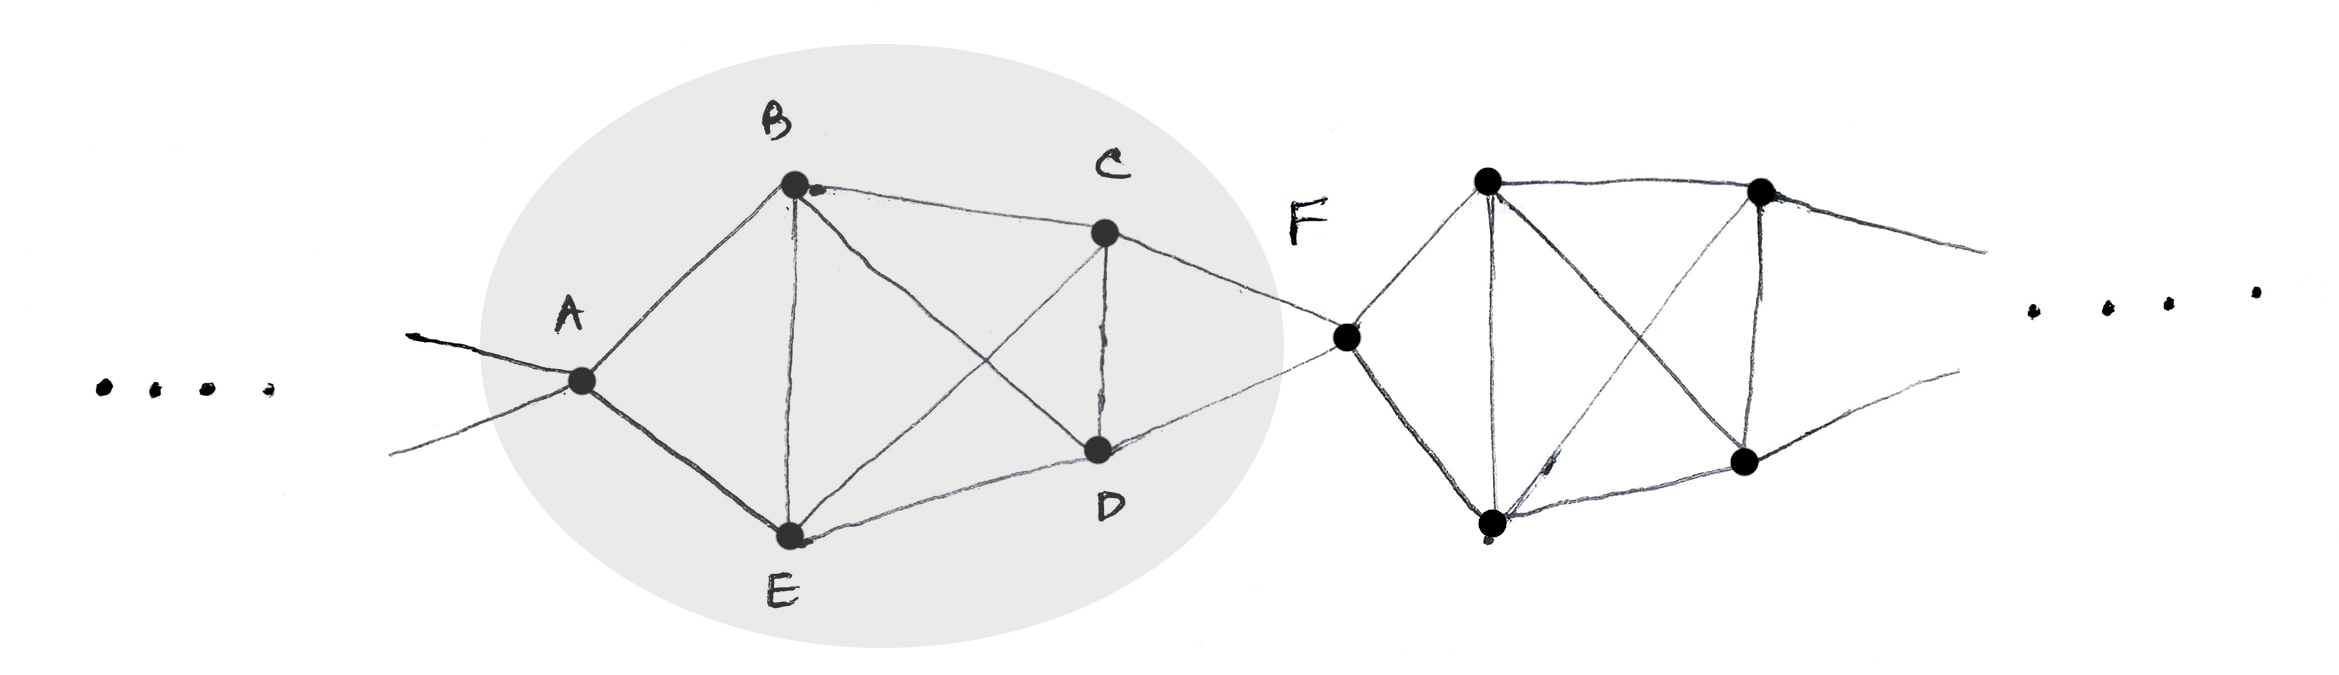
\includegraphics[width=\textwidth]{graph}
%\end{figure}

\begin{center}
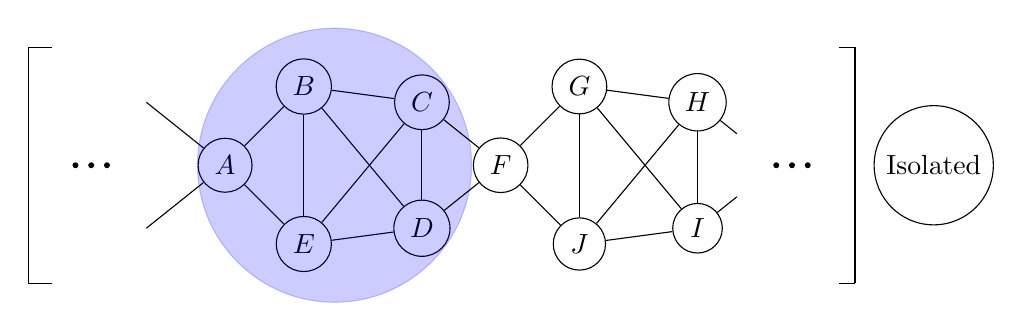
\begin{tikzpicture}[node distance = {15mm}, main/.style = {draw, circle}]

%\foreach \n in {3,...,7}
%  \tikz\foreach \i in {1,...,5}
%    \fill (\i*360/5:1) coordinate (5\i) circle(2 pt)
%      \ifnum \i>1 foreach \j in {\i,...,1}{(5\i) edge (5\j)} \fi;
	
	\draw[-] (-2.5, -1.5) -- (-2.2, -1.5);
	\draw[-] (-2.5, 1.5) -- (-2.2, 1.5);
	\draw[-] (-2.5, -1.5) -- (-2.5, 1.5);
	
	\node[main] (A) at (0, 0) {$A$};
	\node[main] (B) at (1, 1) {$B$};
	\node[main] (C) at (2.5, 0.8) {$C$};
	\node[main] (D) at (2.5, -0.8) {$D$};
	\node[main] (E) at (1, -1) {$E$};
	
	\draw[-] (A) -- (-1, 0.8);
	\draw[-] (A) -- (-1, -0.8);
	
	\draw [draw=black, fill=black] (-1.5,0) circle (0.2ex);
	\draw [draw=black, fill=black] (-1.7,0) circle (0.2ex);
	\draw [draw=black, fill=black] (-1.9,0) circle (0.2ex);
	
	\draw[-] (A) -- (B);
	\draw[-] (A) -- (E);
	\draw[-] (B) -- (E);
	\draw[-] (B) -- (D);
	\draw[-] (B) -- (C);
	\draw[-] (C) -- (D);
	\draw[-] (C) -- (E);
	\draw[-] (D) -- (E);
	
	\draw [draw=blue, fill=blue, opacity=0.2]
       (1.39,0) circle (11.5ex);
	
	\node[main] (A1) at (3.5, 0) {$F$};
	\node[main] (B1) at (4.5, 1) {$G$};
	\node[main] (C1) at (6, 0.8) {$H$};
	\node[main] (D1) at (6, -0.8) {$I$};
	\node[main] (E1) at (4.5, -1) {$J$};
	\draw[-] (C) -- (A1); 
	\draw[-] (D) -- (A1);
	\draw[-] (A1) -- (B1);
	\draw[-] (A1) -- (E1);
	\draw[-] (B1) -- (E1);
	\draw[-] (B1) -- (D1);
	\draw[-] (B1) -- (C1);
	\draw[-] (C1) -- (D1);
	\draw[-] (C1) -- (E1);
	\draw[-] (D1) -- (E1);
	
	\draw[-] (D1) -- (6.5, -0.4);
	\draw[-] (C1) -- (6.5, 0.4);
	
	\draw [draw=black, fill=black] (7,0) circle (0.2ex);
	\draw [draw=black, fill=black] (7.2,0) circle (0.2ex);
	\draw [draw=black, fill=black] (7.4,0) circle (0.2ex);
	
	\draw[-] (8, -1.5) -- (7.8, -1.5);
	\draw[-] (8, 1.5) -- (7.8, 1.5);
	\draw[-] (8, -1.5) -- (8, 1.5);
	
	\node[main] (A2) at (9, 0) {Isolated};
	
\end{tikzpicture}
\end{center}

The following are 10 paths (the remaining 10 are obtained by reflecting the paths over the horizontal axis).

\bgroup
\centering

%\renewcommand{\arraystretch}{2}
\setlength{\tabcolsep}{6mm}
\begin{tabular}{|c|c|c|}
\hline
\begin{tikzpicture}[node distance = {15mm}, main/.style = {draw, circle}]
	\node[main] (A) at (0, 0){};
	\node[main] (B) at (1, 1){};
	\node[main] (C) at (2.5, 1){};
	\node[main] (D) at (2.5, -1){};
	\node[main] (E) at (1, -1){};
	\node[main] (F) at (3.5, 0){};
	\draw[-] (A) -- (B);
	\draw[-] (B) -- (C);
	\draw[-] (C) -- (F); 
	    \addvmargin{2mm}
\end{tikzpicture}
&
\begin{tikzpicture}[node distance = {15mm}, main/.style = {draw, circle}]
	\node[main] (A) at (0, 0){};
	\node[main] (B) at (1, 1){};
	\node[main] (C) at (2.5, 1){};
	\node[main] (D) at (2.5, -1){};
	\node[main] (E) at (1, -1){};
	\node[main] (F) at (3.5, 0){};
	\draw[-] (A) -- (B);
	\draw[-] (B) -- (C);
	\draw[-] (C) -- (D);
	\draw[-] (D) -- (F);
	    \addvmargin{2mm}
\end{tikzpicture}
&
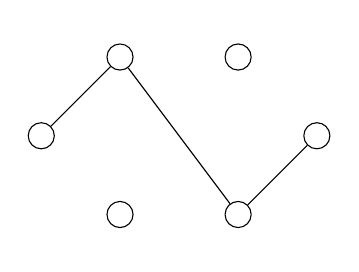
\begin{tikzpicture}[node distance = {15mm}, main/.style = {draw, circle}]
	\node[main] (A) at (0, 0){};
	\node[main] (B) at (1, 1){};
	\node[main] (C) at (2.5, 1){};
	\node[main] (D) at (2.5, -1){};
	\node[main] (E) at (1, -1){};
	\node[main] (F) at (3.5, 0){};
	\draw[-] (A) -- (B);
	\draw[-] (B) -- (D);
	\draw[-] (D) -- (F);
	    \addvmargin{2mm}
\end{tikzpicture}
\\\hline
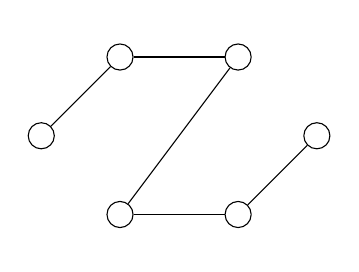
\begin{tikzpicture}[node distance = {15mm}, main/.style = {draw, circle}]
	\node[main] (A) at (0, 0){};
	\node[main] (B) at (1, 1){};
	\node[main] (C) at (2.5, 1){};
	\node[main] (D) at (2.5, -1){};
	\node[main] (E) at (1, -1){};
	\node[main] (F) at (3.5, 0){};
	\draw[-] (A) -- (B);
	\draw[-] (B) -- (C);
	\draw[-] (C) -- (E);
	\draw[-] (D) -- (E);
	\draw[-] (D) -- (F);
	    \addvmargin{2mm}
\end{tikzpicture}
&
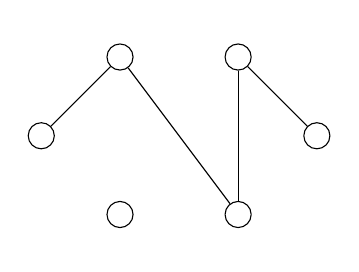
\begin{tikzpicture}[node distance = {15mm}, main/.style = {draw, circle}]
	\node[main] (A) at (0, 0){};
	\node[main] (B) at (1, 1){};
	\node[main] (C) at (2.5, 1){};
	\node[main] (D) at (2.5, -1){};
	\node[main] (E) at (1, -1){};
	\node[main] (F) at (3.5, 0){};
	\draw[-] (A) -- (B);
	\draw[-] (B) -- (D);
	\draw[-] (C) -- (D);
	\draw[-] (C) -- (F);
	    \addvmargin{2mm} 
\end{tikzpicture}
&
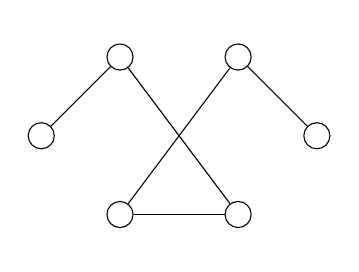
\begin{tikzpicture}[node distance = {15mm}, main/.style = {draw, circle}]
	\node[main] (A) at (0, 0){};
	\node[main] (B) at (1, 1){};
	\node[main] (C) at (2.5, 1){};
	\node[main] (D) at (2.5, -1){};
	\node[main] (E) at (1, -1){};
	\node[main] (F) at (3.5, 0){};
	\draw[-] (A) -- (B);
	\draw[-] (B) -- (D);
	\draw[-] (C) -- (E);
	\draw[-] (D) -- (E);
	\draw[-] (C) -- (F);
	    \addvmargin{2mm} 
\end{tikzpicture}
\\\hline
\begin{tikzpicture}[node distance = {15mm}, main/.style = {draw, circle}]
	\node[main] (A) at (0, 0){};
	\node[main] (B) at (1, 1){};
	\node[main] (C) at (2.5, 1){};
	\node[main] (D) at (2.5, -1){};
	\node[main] (E) at (1, -1){};
	\node[main] (F) at (3.5, 0){};
	\draw[-] (A) -- (B);
	\draw[-] (B) -- (E);
	\draw[-] (D) -- (E);
	\draw[-] (D) -- (F);
	    \addvmargin{2mm}
\end{tikzpicture}
&
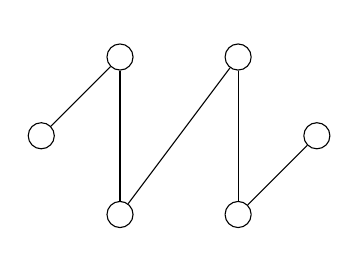
\begin{tikzpicture}[node distance = {15mm}, main/.style = {draw, circle}]
	\node[main] (A) at (0, 0){};
	\node[main] (B) at (1, 1){};
	\node[main] (C) at (2.5, 1){};
	\node[main] (D) at (2.5, -1){};
	\node[main] (E) at (1, -1){};
	\node[main] (F) at (3.5, 0){};
	\draw[-] (A) -- (B);
	\draw[-] (B) -- (E);
	\draw[-] (C) -- (D);
	\draw[-] (C) -- (E);
	\draw[-] (D) -- (F);
	    \addvmargin{2mm}
\end{tikzpicture}
&
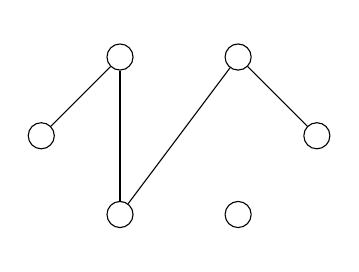
\begin{tikzpicture}[node distance = {15mm}, main/.style = {draw, circle}]
	\node[main] (A) at (0, 0){};
	\node[main] (B) at (1, 1){};
	\node[main] (C) at (2.5, 1){};
	\node[main] (D) at (2.5, -1){};
	\node[main] (E) at (1, -1){};
	\node[main] (F) at (3.5, 0){};
	\draw[-] (A) -- (B);
	\draw[-] (B) -- (E);
	\draw[-] (C) -- (E);
	\draw[-] (C) -- (F);
	    \addvmargin{2mm} 
\end{tikzpicture}
\\\hline
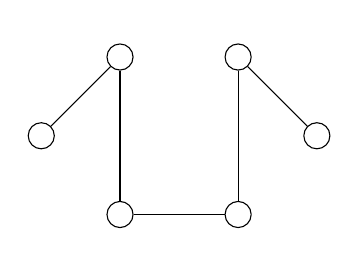
\begin{tikzpicture}[node distance = {15mm}, main/.style = {draw, circle}]
	\node[main] (A) at (0, 0){};
	\node[main] (B) at (1, 1){};
	\node[main] (C) at (2.5, 1){};
	\node[main] (D) at (2.5, -1){};
	\node[main] (E) at (1, -1){};
	\node[main] (F) at (3.5, 0){};
	\draw[-] (A) -- (B);
	\draw[-] (B) -- (E);
	\draw[-] (C) -- (D);
	\draw[-] (D) -- (E);
	\draw[-] (C) -- (F);
	    \addvmargin{2mm} 
\end{tikzpicture}\\
\cline{1-1}
\end{tabular}
\egroup

\end{solution}


\vspace{0.3in}




\question[20] Design an $O(poly(n) \cdot 2^{n/4})$-time backtracking algorithm for the maximum independent set problem for graphs with bounded degree $3$ (these are graphs where all vertices have degree at most $3$). Give running time analysis and proof of correctness.

\begin{solution}

    Note that the following algorithm also works for graphs with vertices with degree more than $3$, however the exhibited runtime bound matches with the requested runtime bound only for graphs with bounded degree $3$.

    We exhibit an algorithm that works in $O((n + m)^2 2^{n'/4})$ time, where $m$ is the number of edges in the graph, and $n'$ is defined as $$\sum_{i \in \mathbb{N}} i \times\text{number of vertices with degree }(i + 2)$$
    Clearly for a graph with max degree $3$, we have $n' \le n$, and $m = O(n)$, so the algorithm has runtime in $O(n^2 2^{n/4})$. 

    \textbf{Note:} The following algorithm can be optimized in a real-world implementation using backtracking and updating the graph instead of creating a new graph each time, and maintaining a heap
    to find the vertex with the least degree. However, the complexity still remains the same and there is no real complexity gain.

    Denote by $N(v)$ the neighbours of a vertex $v$ for the sake of brevity. Edges are denoted as ordered pairs $\{u, v\}$ and not as ordered pairs $(u, v)$ since the graph is undirected.

\paragraph{Algorithm}

\begin{algorithmic}[1]
\Function{MaximumIndependentSet}{Graph $G = (V, E)$}
    \If{$G$ is empty}
        \State \Return $\{\}$
    \EndIf
    \State \textbf{let} $v$ be the vertex with the least degree in $G$
    \If{$deg(v) = 0$}
        \State \Return $\{v\}\, \cup\, $\textsc{MaximumIndependentSet}$(G \setminus \{v\})$
    \ElsIf{$deg(v) = 1$}
        \State \textbf{let} $u$ be the (only) neighbour of $v$
        \State \Return $\{v\}\, \cup\, $\textsc{MaximumIndependentSet}$(G \setminus \{v, u\})$
    \ElsIf{$deg(v) = 2$}
        \State \textbf{let} $u_1, u_2$ be the (only) neighbours of $v$.
        \If{there is an edge between $u_1$ and $u_2$ in $G$}
            \State \Return $\{v\}\, \cup\,$ \textsc{MaximumIndependentSet}$(G \setminus \{v, u_1, u_2\})$
        \Else
            \State \textbf{let} $v'$ be a new vertex not in $G$.
            \State \textbf{let} $E_o = \{\{u_1, u\} \mid u \in N(u_1)\} \cup \{\{u, u_2\} \mid u \in N(u_2)\}$ \Comment{Edges incident to at least one vertex in the set $\{u_1, u_2\}$. Recall that we represent edges as unordered pairs.}
            \State \textbf{let} $E_n = \{\{v', u\} \mid u \in N(u_1) \cup N(u_2) \setminus \{v\}\}$ \Comment{Edges that will join $v'$ to all neighbours of $u_1, u_2$ except $v$}
            \State \textbf{let} $G' = ((V \cup \{v'\}) \setminus \{v, u_1, u_2\}, (E \cup E_n) \setminus E_o)$ \Comment{Merge $v, u_1, u_2$ into `super-node' $v'$}
            \State \textbf{let} $S = \,$ \textsc{MaximumIndependentSet}$(G')$.
            \If{$v'$ is in $S$}
                \State \Return $\{u_1, u_2\}\, \cup\, S \setminus \{v'\}$ 
            \Else
                \State \Return $\{v\}\, \cup\, S$
            \EndIf
        \EndIf
    \Else \Comment{In this case, $deg(v) \ge 3$}
        \State \textbf{let} $S_1 = \{v\}\, \cup\,$\textsc{MaximumIndependentSet}$(G \setminus (\{v\} \cup N(v)))$
        \State \textbf{let} $S_2 =\, $\textsc{MaximumIndependentSet}$(G \setminus \{v\})$ 
        \State \Return the larger of $S_1, S_2$.
    \EndIf
\EndFunction
\end{algorithmic}

\paragraph{Proof of Correctness} We prove the correctness of the algorithm using induction on the number of vertices in the graph.\nl
\textbf{Inductive hypothesis:} \textsc{MaximumIndependentSet}$(G)$ returns a maximum independent set of $G$ for all graphs $G$ with number of vertices less than $n$ for some $n > 0$.\nl
\textbf{Base Case:} In the case the graph is empty, the maximum independent set of the graph is the empty set, and hence the algorithm returns the correct answer in the case that the graph is empty.\nl
\textbf{Inductive step:}\nl
Firstly we claim the following:

    \begin{claim}
        For any graph $G$, and a vertex $v$ in it, if there is a maximum independent set in $G$ that contains exactly one vertex in $\{v\} \cup N(v)$, then there is a maximum independent set in
        $G$ containing $v$.
    \end{claim}

    \begin{proof}
        Suppose that there exists a maximum independent set $S$ in $G$ that contains exactly one vertex out of the vertices in $\{v\} \cup N(v)$. If that vertex is $v$, we are trivially done. Now
        assume that $S$ contains a vertex in $N(v)$, say $u$. Consider the set $S \setminus \{u\} \cup \{v\}$. Note that since there is no neighbour of $v$ in this set (which is because $u$ was the
        only neighbour of $v$ in $S$), this set is also a valid independent set by the validity of $S$ and this observation. Since the size of this set is the same as that of $S$, this set is also a
        maximum independent set in $G$, and we have shown the claim, as needed.
    \end{proof}

Now, we make cases on the vertex $v$ with the least degree in the graph.

\begin{enumerate}
    \item $deg(v) = 0$.\nl
    In this case, since this vertex is isolated, we claim that this vertex will always be in any maximum independent set of $G$. Indeed, suppose $S$ is any maximum independent set of $G$ that doesn't
        contain $v$. Then for any vertex $u$ in $S$, since $deg(v) = 0$, $u$ is not adjacent to any vertex in $S$. Hence we can add $u$ to $S$ to get a bigger independent set, which is a
        contradiction. By the inductive hypothesis, the recursive call gives the rest of the independent set, as needed.
    \item $deg(v) = 1$.\nl
    We claim that there is always at least one maximum independent set of $G$ that contains $v$. Let $u$ be the only neighbour of $v$. Consider any maximum independent set $S$ of $G$.
    \begin{enumerate}
        \item $S$ contains at least one of $u, v$.\nl
        Note that it can't contain both of these vertices. Also, by the claim in the beginning, we have a maximum independent set that contains $v$.
        \item $S$ contains none of $u, v$.\nl
        By a completely similar analysis, we can show that $S \cup \{v\}$ is also an independent set, which is larger than $S$, and it contradicts the fact that $S$ is a maximum independent set of $G$.
    \end{enumerate}
    Hence, we have shown our claim, so it is always optimal to choose a degree $1$ vertex. Since $u$ can't be in such an independent set, the remaining part of the set must come from $G \setminus \{u,
        v\}$, and must be independent. Note that the maximum independent set of this subgraph is an independent set by definition, and taking the union of this with $v$ yields an independent set of
        $G$. It is also the maximum independent set of $G$, since if it wasn't, then removing the vertex $v$ from the maximum independent set of $G$ which has $v$ would yield a larger independent set
        of $G \setminus \{u, v\}$. By the induction hypothesis, the recursive call in the function corresponding to this case gives a maximum independent set of this case, and we are done in this
        case.
    \item $deg(v) = 2$.\nl
        Let $u_1, u_2$ be the two neighbours of $v$.
        In this case, we make two subcases:
        \begin{enumerate}
            \item There is an edge between $u_1, u_2$. In this case, we can choose exactly one of $v, u_1, u_2$ in the maximum independent set (if we choose none, the maximum property is violated by
                adding in $v$, and if we choose two or more, the set is no longer independent). By the claim, it is optimal to choose $v$, and the remaining set must come from $G \setminus \{v,
                u_1, u_2\}$. Using a completely analogous argument as in the degree 1 case, we can show that the union of the chosen vertex (which is $v$) and the answer of the recursive call is a
                maximum independent set of the graph.
            \item There is no edge between $u_1, u_2$. In this case, we can choose either one or two vertices from $\{v, u_1, u_2\}$ in the maximum independent set of $G$. We combine the nodes $v,
                u_1, u_2$ into a node $v'$ to get a new graph $G'$. Note that the recursive call computes a maximum independent set of this new graph since it has two less vertices than $G$, call that set $S$.
                Our claim is the following:
                \begin{claim}
                    If $S$ contains $v'$, then it is optimal to choose $u_1, u_2$ in $G$, and if $S$ doesn't contain $v$, then it is optimal to choose $v$ in $G$.
                \end{claim}
                \begin{proof}
                We first show how to construct an independent set of $G$ from $S$ which has exactly one more vertex than $S$.
                We make two cases:
                    \begin{enumerate}
                        \item $S$ contains $v'$.\nl
                            Note that since $S$ contains $v'$, no vertex adjacent to $v'$ in $G'$ is in $S$, and thus no neighbour of $u_1, u_2$ is in $S$. Hence we can add $u_1, u_2$ after removing
                            $v'$ to get an independent set of $G$ with exactly one more vertex than $S$ has.
                        \item $S$ doesn't contain $v'$.\nl
                            In this case, we can add $v$ to $S$, and this is an independent set because no neighbour of $v$ is in $S$. Since we have added one vertex to $S$, the size of this set
                            is exactly one more than that of $S$.
                    \end{enumerate}
                Now we show that the size of any independent set $S'$ of $G$ is at most $1 + |S|$.
                We make two cases again:
                    \begin{enumerate}
                        \item At least two of $v, u_1, u_2$ are in $S'$.\nl
                            In this case, since $v$ is adjacent to $u_1, u_2$, so $v$ can't be in $S'$. Hence $u_1, u_2$ are both in $S$. Consider the corresponding independent set in $G'$ (formed
                            by choosing the vertices in $S'$ except $u_1, u_2$ but possibly also containing $v'$ -- the set without $v'$ is independent because of being a subset of $S'$, but as
                            we show in the next sentence, we can choose $v'$ as well and still have this set as independent in $G'$). Note
                            that since $u_1, u_2$ have both been chosen, $v'$ has been chosen in the corresponding independent set in $G'$ (since the neighbours of $v'$ are precisely the neighbours of
                            $u_1, u_2$ except $v$, and none of them have been chosen in $S'$ because $u_1, u_2$ have been chosen), so we have an independent set of size $|S'| - 1$ in $G'$. Now that we know that the maximum size of an
                            independent set in $G'$ is $|S|$, we have $|S'| - 1 \le |S|$, or $|S'| \le 1 + |S|$, as needed.
                        \item Exactly one of $v, u_1, u_2$ is in $S'$.\nl
                            Again, considering the corresponding independent set in $G'$, either $v'$ is chosen or it is not, and in either case, we have that the size of that set is either
                            $|S'|$ or $|S'| - 1$. Since the size of the corresponding independent set is at most $|S|$ (as $S$ is a maximum independent set of $G'$), $|S'|$ is at most $\max(|S|,
                            |S| + 1)$, so we have $|S'| \le |S| + 1$ in this case as well.
                    \end{enumerate}
                From this analysis, we see that any independent set of $G$ must have at most $|S| + 1$ vertices. Since we have exhibited an independent set of $G$ with exactly these many vertices,
                    it must be a maximum independent set of $G$ in each case.
                \end{proof}
            Note that this finishes the proof of the claim, and thus by the claim (and the construction mentioned in the proof), the independent set returned by the algorithm is indeed a
                maximum independent set of $G$.
      \end{enumerate}
  \item $deg(v) \ge 3$.\nl
      In this case, either we choose $v$ or not. If we choose $v$, the answer is the union of $v$ with the maximum independent set of the graph obtained after we remove $v$ and all its three
      neighbours, and if we don't, then the answer is the union of $v$ with the maximum independent set of the graph obtained after we remove $v$ from $G$, as done in class. Since both of these graphs
      have number of vertices strictly less than that of $G$, using the inductive hypothesis, we are done in this case as well.
\end{enumerate}

By the above case analysis, we can see that the algorithm returns a maximum independent set in all cases, and thus the induction is complete.

\paragraph{Time complexity analysis} Let $n, m$ be the number of nodes, edges in the graph, and let $n'$ be as defined. Let the number of constant-time operations
needed in this algorithm be denoted by $f(n, m, n')$. Then we claim that $f(n, m, n') \le c (n + m + 1)^2 2^{n'/4}$ for any non-empty graph where $c$ is a suitably chosen large enough constant, which will be specified later on.

We first begin with two claims:

\begin{claim}
    $n' = \sum_{v \in V(G)} \max(0, deg(v) - 2)$.
\end{claim}
\begin{proof}
    Note that for each vertex with degree $i$ contributes $i - 2$ to the right hand side if $i \ge 3$ and $0$ otherwise. Hence by grouping vertices by degree, we have the result. More precisely, we
    have:
    \begin{align*}
        \sum_{v \in V(G)} \max(0, deg(v) - 2)
           &= \sum_{j \in \mathbb{N}}\sum_{v \in V(G), deg(v) = j} \max(0, j - 2)\\
           &= \sum_{j \in \mathbb{N}_{\ge 3}}\sum_{v \in V(G), deg(v) = j} (j - 2)\\
           &= \sum_{i \in \mathbb{N}} \sum_{v \in V(G), deg(v) = i + 2} i\\
           &= \sum_{i \in \mathbb{N}} i \times |\{v \in V(G) \mid deg(v) = i + 2\}|\\
           &= n'
    \end{align*}
    as required.
\end{proof}

\begin{claim}
    Whenever we create a graph $G'$ from $G$ in the algorithm, $n'(G') \le n'(G)$.
\end{claim}
\begin{proof}
    Note that in the cases with minimum degree 0, 1, or at least 3, we always remove vertices from the graph, which either reduces the degree of any remaining vertex or keeps it the same, and also removes the non-negative contribution of the removed vertices from the expression of $n'$. Hence the inequality holds in that case. The same holds in the subcase of the case of minimum degree 2 where we have an edge between $u_1, u_2$.\nl
    The more important case is when the minimum degree is $2$ and we replace a group of nodes with a new node.\nl
    In the case when the degree is $2$, the highest possible degree of the combined node is $deg(u_1) + deg(u_2) - 2$ (this is in the case when $N(u_1), N(u_2)$ intersect in only one vertex $v$). The contribution of $v, u_1, u_2$ to $n'(G)$ is $0, \max(deg(u_1) - 2, 0), \max(deg(u_2) - 2, 0)$ respectively. Also, for any vertex adjacent to both $u_1, u_2$, its degree in the new graph is one less than its old degree, and this can't increase the difference between $n'(G'), n'(G)$. Hence we have 
    $$n'(G') - n'(G) \le \max(deg(u_1) + deg(u_2) - 4, 0) - \max(deg(u_1) - 2, 0) - \max(deg(u_2) - 2, 0)$$
    
    Note that the real function $f(a) = \max(a, 0)$ is the point-wise maximum of the identity function and the 0 function, both of which are convex, and hence it is also convex. So it satisfies $f(a) + f(b) \ge 2f\left(\frac{a + b}{2}\right)$ (special case of Jensen's inequality), and thus applying this inequality to $(a, b) = (deg(u_1) - 2, deg(u_2) - 2)$, we have that 
    \begin{align*}
        n'(G') - n'(G) &\le \max(deg(u_1) + deg(u_2) - 4, 0) - \max(deg(u_1) - 2, 0) - \max(deg(u_2) - 2, 0)\\
                       &= 2 \max\left(\frac{deg(u_1) + deg(u_2) - 4}{2}, 0\right) - \max(deg(u_1) - 2, 0) - \max(deg(u_2) - 2, 0)\\
                       &\le 0
    \end{align*}
    This completes the proof.
\end{proof}

Now we move to the main proof of the time complexity.

\textbf{Note that all the constants $c_i$ mentioned in the below proof shall be such that the mentioned upper bound holds for all $n$, and not just the particular $n$ considered in the
inductive step.}

\begin{proof}
    The proof goes by strong induction on the lexicographical ordering of tuples $(n, m, n')$ of non-negative integers.\nl
    For the base case, if the number of operations to check if the graph is empty is $c_1$, then if we have $c \ge c_1$, the base case holds.\nl
    The number of operations to find out the vertex with the least degree is at most linear in $n + m$. Suppose it is upper bounded by
    $c_2(n + m)$ for all $n, m$.\nl
    If the degree is $0$, then removing the vertex from the graph takes at most linear operations (wherever operations are mentioned, we mean constant-time operations unless specified otherwise).
    Suppose the time for this and taking the union and returning the set is upper bounded by $c_3(n + m)$ for all $n, m$. So we have 
    \begin{align*}
        f(n, m, n') &\le f(n - 1, m, n') + c_3 n + c_2 n\\
        &\le c(n + m)^2 2^{n'/4} + (c_3 + c_2)(n + m)\\
        &\le c(n + m + 1)^2 2^{n' / 4}
    \end{align*}
        where the last inequality is true if we have $c > c_3 + c_2$.\nl
    If the degree is $1$, then removing both vertices and returning the set takes linear time, say upper bounded by $c_4(n + m)$ for all $n, m$. Then we have \begin{align*}
        f(n, m, n') &\le \max_{0 \le i \le n'}f(n - 2, m - \deg(u), n' - i) + (c_4 + c_2)(n + m)\\
        &\le c(n + m - 1)^2 2^{n'/4} + (c_4 + c_2)(n + m)\\
        &\le c(n + m + 1)^2 2^{n'/4}
\end{align*}
    where the last inequality is true if we have $c > c_4 + c_2$.\nl
    If the degree is $2$, the checking of the two subcases takes at most linear number of operations, upper bounded by, say $c_5(n + m)$ for all $n, m$.
    
    In the first subcase, the removal of the vertices to get a new graph, taking the union and returning takes at most $c_6(n + m)$ operations for all $n, m$, for some constant $c_6$. Then we have 
    \begin{align*}
        f(n, m, n') &\le \max_{0 \le i \le n'}f(n - 3, m - 3 - \epsilon, n' - i) + (c_6 n + c_5 + c_2)(n + m)\\
                &\le c(n + m - 5)^2 2^{n'/4} + (c_6 n + c_5 + c_2)(n + m)\\
                &\le c(n + m - 5)^2 2^{n'/4} + (c_6 n + c_5 + c_2)(n + m)\\
                &\le c(n + m + 1)^2 2^{n'/4}
    \end{align*}
    where the last inequality is true if $c > c_5 + c_6 + c_2$.
    
    In the second subcase, the creation of the new graph takes a linear number of operations, and so does taking the union, searching in the returned set, modifying the returned set and returning it.
    Suppose it is upper bounded by $c_7(n + m)$ for all $n, m$.
    \begin{align*}
        f(n, m, n') &\le \max_{0 \le i \le n'}f(n - 2, m - 2 - \epsilon, n' - i) + (c_7 + c_5 + c_2)(n + m)\\
                &\le c(n + m - 3)^2 2^{n'/4} + (c_7 + c_5 + c_2)(n + m)\\
                &\le c(n + m + 1)^2 2^{n'/4}
    \end{align*}
    where the last inequality is true if $c > c_7 + c_5 + c_2$.

    If none of the above cases is true, then the minimum degree $d$ in the graph must be at least $3$, and as a consequence, all vertices in the graph must have degree at least $d$.
    Comparing sizes of sets and returning the larger one of them takes linear number of operations, and so does creating two graphs with one and two vertices removed. 
    Suppose all of this is upper bounded by $c_8 (n + m)$ for all $n, m$.

    We compute the difference in $n'$ in this case. When we remove a vertex with degree $d$, $n'$ decreases by at least $2d - 2$, since the contribution of this vertex is $d - 2$, and the reduction
    in the degree of each other vertex is exactly $1$. 
    When we remove this vertex and the set of all neighbours of this vertex, the reduction in $n'$ is at least $(d + 1)(d - 2)$. Let the exact reduction be $d'$. 

    We then have:
    \begin{align*}
        f(n, m, n') &\le f(n - 1, m - d, n' - 2d + 2) + f(n - d - 1, m - d - \epsilon, n' - d') + (c_8 + c_2)(n + m)\\
                &\le cn^2 2^{(n' - 2d + 2) / 4} + c(n - d)^2
    2^{(n' - d') / 4} + c_8 n + c_2 n \\
                &\le c(n + m - d)^2 2^{(n' - 2d + 2) / 4} + c(n + m - 2d)^2 2^{(n' - (d+1)(d-2)) / 4} + (c_8 + c_2)(n + m) \\
                &\le c(n + m - 3)^2 2^{(n' - 4) / 4} + c(n + m - 6)^2 2^{(n' - 4) / 4} + (c_8 + c_2)(n + m)\\
                &= \frac{1}{2} \cdot c(n + m - 3)^2 2^{n' / 4} + \frac{1}{2} \cdot c(n + m - 6)^2 2^{n' / 4} + (c_8 + c_2)(n + m)\\
                &\le \frac{1}{2} \cdot c(n + m)^2 2^{n'/4} + \frac{1}{2} \cdot c(n + m)^2 2^{n'/4} + (c_8 + c_2)(n + m)\\
                &= c(n + m)^2 2^{n'/4} + (c_8 + c_2)(n + m)\\
                &\le c(n + m + 1)^2 2^{n'/4}
    \end{align*}
    where the last inequality is true if $c > c_8 + c_2$. We have made use of the facts that $d \ge 3$, $d' \ge 4d - 8$, and that $(d + 1)(d - 2)$ is increasing on $[2, \infty)$.

    Note that if we choose $c = 1 + c_2 + \max(c_1 - c_2, c_3, c_4, c_5 + c_6, c_5 + c_7, c_8)$, all of these claims will be valid, and thus our proof by induction is complete.
\end{proof}

Since our claim is completed, we have that for $n > 0$, our algorithm takes $O((n + m + 1)^2 2^{n'/4})$ time, since it takes the same order of constant time operations.
Note that we have $n' \le n$ as well as $m = O(n)$ for any graph with bounded degree 3, so the runtime of the algorithm is in $O(n^2 2^{n / 4})$, as required.

\end{solution}

\end{questions}
\end{document}
